% ============================================================================
% End-Semester Review Presentation (Beamer 16:9, navy theme of the mid-review).
% Numbers identical to main_v2.tex (verified against source files).
% Build: pdflatex presentation_final.tex (twice)
% ============================================================================
\documentclass[aspectratio=169,10pt]{beamer}
\usetheme{Madrid}
\usepackage[utf8]{inputenc}
\usepackage[T1]{fontenc}
\usepackage{booktabs,array,tabularx,multicol}
\usepackage{graphicx}
\graphicspath{{./}{figures/}}

% ---- colours ---------------------------------------------------------------
\definecolor{navy}{HTML}{14325F}
\definecolor{navy2}{HTML}{2A5F9E}
\definecolor{soft}{HTML}{F4F6FA}
\definecolor{gapred}{HTML}{B22222}
\definecolor{good}{HTML}{1E7B34}
\setbeamercolor{structure}{fg=navy}
\setbeamercolor{frametitle}{bg=navy,fg=white}
\setbeamercolor{block title}{bg=navy,fg=white}
\setbeamercolor{block body}{bg=soft,fg=black}
\setbeamercolor{block title alerted}{bg=gapred,fg=white}
\setbeamercolor{block body alerted}{bg=soft,fg=black}
\setbeamercolor{block title example}{bg=good,fg=white}
\setbeamercolor{block body example}{bg=soft,fg=black}
\setbeamercolor{title}{bg=navy,fg=white}
\setbeamertemplate{blocks}[rounded][shadow=true]
\setbeamertemplate{navigation symbols}{}
\setbeamertemplate{itemize item}{\color{navy2}$\bullet$}
\setbeamertemplate{itemize subitem}{\color{navy2}--}
\setbeamerfont{frametitle}{size=\large}
\setbeamerfont{block title}{size=\small}

% frame title: full-width navy bar + logo at the right
\setbeamertemplate{frametitle}{%
  \nointerlineskip
  \begin{beamercolorbox}[wd=\paperwidth,ht=2.6ex,dp=1.2ex,leftskip=0.6cm,rightskip=0.3cm]{frametitle}
    \usebeamerfont{frametitle}\insertframetitle\hfill
    \raisebox{-0.55ex}{
\includegraphics[height=3.4ex]{figures/logo.jpeg}}
  \end{beamercolorbox}\vspace{1mm}}

% footer
\setbeamertemplate{footline}{%
  \leavevmode\hbox{%
  \begin{beamercolorbox}[wd=.30\paperwidth,ht=2.4ex,dp=1ex,leftskip=0.4cm]{author in head/foot}%
    \usebeamerfont{author in head/foot}\textbf{IIITDM Kurnool} \;|\; Dept.\ of CSE
  \end{beamercolorbox}%
  \begin{beamercolorbox}[wd=.50\paperwidth,ht=2.4ex,dp=1ex,center]{title in head/foot}%
    \usebeamerfont{title in head/foot}Multimodal Agricultural Drought Monitoring and Prediction
  \end{beamercolorbox}%
  \begin{beamercolorbox}[wd=.20\paperwidth,ht=2.4ex,dp=1ex,right,rightskip=0.4cm]{date in head/foot}%
    \usebeamerfont{date in head/foot}November 2026 \quad \insertframenumber{} / \inserttotalframenumber
  \end{beamercolorbox}}}
\setbeamercolor{author in head/foot}{bg=navy,fg=white}
\setbeamercolor{title in head/foot}{bg=navy2,fg=white}
\setbeamercolor{date in head/foot}{bg=navy,fg=white}

\newcolumntype{Y}{>{\raggedright\arraybackslash}X}
\newcommand{\key}[2]{{\color{navy}\bfseries\Large #1}\\[-1pt]{\scriptsize #2}}
\setlength{\tabcolsep}{4pt}

\begin{document}

% ============================================================ 1 TITLE
\begin{frame}[plain]
\centering
\vspace{2mm}

\includegraphics[height=1.55cm]{figures/logo.jpeg}\\[1mm]
{\small\bfseries INDIAN INSTITUTE OF INFORMATION TECHNOLOGY DESIGN AND MANUFACTURING KURNOOL}\\[3mm]
\begin{beamercolorbox}[wd=0.94\paperwidth,sep=7pt,rounded=true,shadow=true,center]{title}
{\large\bfseries A Multimodal Framework for Agricultural Drought Monitoring and Prediction\\
using Weather Time Series, Satellite Imagery, and UAV Semantic Segmentation}\\[4pt]
{\normalsize End-Semester Review Presentation}
\end{beamercolorbox}\par\vspace{4mm}
{\small\bfseries Presented by:}\\[1mm]
{\small\textbf{G. Aryan Rajesh} (123CS0020) \quad \textbf{M. Rovan} (123CS0036) \quad \textbf{M. Harsha Vardhan} (123CS0044)}\\[3mm]
{\small\bfseries Under the Guidance of:}\\[1mm]
{\normalsize\bfseries Dr. M. NARESH BABU}\\
{\small Associate Professor, Dept.\ of CSE}\\[3mm]
{\small Department of Computer Science and Engineering \quad $\cdot$ \quad November 2026}
\end{frame}

% ============================================================ 3 INTRODUCTION
\begin{frame}{1. Introduction: Agricultural Drought in Rayalaseema}
\begin{columns}[T]
\column{0.53\textwidth}
\begin{block}{The regional problem}
\footnotesize
\begin{itemize}
\item Rayalaseema (Kurnool, Anantapur, Sri Sathya Sai) and Tumakuru: low, erratic rainfall.
\item \textbf{Kharif} (Jun--Nov) crops depend on the monsoon; \textbf{rabi} (Oct--Apr) crops on stored soil water.
\item Drought is declared by Government Orders (G.O.s) \textbf{late in the season}; detection is weakest in AP and Karnataka.
\item Weather, satellite and drone studies are usually done \textbf{separately}.
\end{itemize}
\end{block}
\begin{block}{Our idea}
\footnotesize \textbf{Weather predicts} where to look $\rightarrow$ \textbf{satellite confirms} which fields are stressed $\rightarrow$ \textbf{drone measures} the damage --- in \textbf{both seasons}.
\end{block}
\column{0.44\textwidth}
\begin{block}{8 study sites (6 independent weather cells)}
\footnotesize
\begin{tabular}{@{}ll@{}}
\textbf{Somandepalle} (Sri Sathya Sai) & 13.999N, 77.625E \\
\textbf{Lepakshi} (Sri Sathya Sai) & 13.800N, 77.619E \\
\textbf{Cholasamudram} (Sri Sathya Sai) & 13.812N, 77.569E \\
\textbf{Sira} (Tumakuru, KA) & 13.798N, 76.975E \\
\textbf{Peddakadubur} (Kurnool) & 15.783N, 77.253E \\
\textbf{Dinnedevarapadu} (Kurnool) & 15.772N, 78.047E \\
\textbf{Balaji Villas} (Kurnool) & 15.783N, 78.056E \\
\textbf{Pullaiah College} (Kurnool) & 15.798N, 78.081E \\
\end{tabular}\\[3pt]
Each site is a UAV survey field.
\end{block}
\end{columns}
\end{frame}

% ============================================================ 4 GAPS
\begin{frame}{2. Research Gaps and Our Solutions}
\begin{columns}[T]
\column{0.49\textwidth}
\begin{alertblock}{Gap 1 -- Weak forecast evaluation}
\footnotesize Drought indices are often calibrated on the full record (test years leak into labels) and models are compared only with other ML models.\\[2pt]
\textcolor{good}{\textbf{Ours:}} SPEI frozen on 1979--2011; baselines include persistence and a physical water-balance model.
\end{alertblock}
\begin{alertblock}{Gap 2 -- Index-vs-index validation}
\footnotesize Satellite studies validate one index against another at coarse scale.\\[2pt]
\textcolor{good}{\textbf{Ours:}} 240 random 10\,m fields; live replay against 4 seasons of government orders with real data delays.
\end{alertblock}
\column{0.49\textwidth}
\begin{alertblock}{Gap 3 -- Rabi drought unchecked}
\footnotesize Rabi drought is assessed after the season with rain indices rarely checked against crop outcomes.\\[2pt]
\textcolor{good}{\textbf{Ours:}} soil-moisture deficit indicator validated against district crop yields (1997--2022).
\end{alertblock}
\begin{alertblock}{Gap 4 -- UAV not scalable, modules not linked}
\footnotesize UAV studies classify small images, do not report areas, and are not linked to weather or satellite.\\[2pt]
\textcolor{good}{\textbf{Ours:}} 7-class segmentation of 2.9-billion-pixel orthomosaics with m$^2$ areas; kharif and rabi hand fields to the drone.
\end{alertblock}
\end{columns}
\end{frame}

% ============================================================ 5 PROBLEM / OBJECTIVES
\begin{frame}{3. Problem Statement and Objectives}
\begin{block}{Problem statement}
\footnotesize Using daily weather (1979--2026), satellite imagery (2000--2026) and drone imagery for 8 agricultural sites in Kurnool, Sri Sathya Sai (Andhra Pradesh) and Tumakuru (Karnataka), build and honestly evaluate a framework that \textbf{forecasts} drought, \textbf{confirms} it on crops and \textbf{measures} it on fields, in both the kharif and rabi seasons.
\end{block}
\begin{columns}[T]
\column{0.49\textwidth}
\begin{block}{O1 -- Weather forecast}
\footnotesize Forecast the SPEI-30 drought class (healthy / moderate / severe) 7, 15 and 30 days ahead and beat persistence and a physical water-balance model.
\end{block}
\begin{block}{O2 -- Satellite confirmation}
\footnotesize Confirm crop stress on randomly sampled Sentinel-2 fields and replay the chain against government drought orders with real data delays.
\end{block}
\column{0.49\textwidth}
\begin{block}{O3 -- Rabi drought}
\footnotesize Build a rabi drought indicator from root-zone soil moisture and validate it against district crop yields.
\end{block}
\begin{block}{O4 -- UAV segmentation}
\footnotesize Segment drone orthomosaics into 7 classes (soil, crop, cotton boll, green weed, dry weed, drought, background) and estimate class areas in m$^2$.
\end{block}
\begin{block}{O5 -- Integration}
\footnotesize Connect the modules: kharif and rabi outputs list the fields to survey with the drone.
\end{block}
\end{columns}
\end{frame}

% ============================================================ 6 DATA + ARCHITECTURE
\begin{frame}{4. Data Sources and Overall Architecture}
\begin{columns}[T]
\column{0.47\textwidth}
\begin{block}{Data (all public or collected; nothing simulated)}
\scriptsize
\renewcommand{\arraystretch}{1.2}
\begin{tabularx}{\linewidth}{@{}p{2.3cm}Yp{1.3cm}@{}}
\toprule
\textbf{Source} & \textbf{Content} & \textbf{Period} \\ \midrule
AgERA5 & daily rain, ET$_0$, temp., humidity, wind, radiation & 1979--2026 \\
Sentinel-2 (Earth Engine) & 10\,m NDVI, 240 fields + 1,350 rabi points & 2019--2026 \\
ERA5-Land & root-zone soil moisture, 45 points & 1990--2023 \\
MODIS MOD13Q1 & 250\,m NDVI on cropland & 2000--2026 \\
District crop statistics & rabi yield of all crops & 1997--2022 \\
Drought G.O.s & declared mandals (comparison only) & 2023--2026 \\
UAV surveys (Dr.\ Naresh Babu \& team) & 14 orthomosaics & Nov 2025 -- Jan 2026 \\
\bottomrule
\end{tabularx}
\end{block}
\column{0.5\textwidth}
\centering
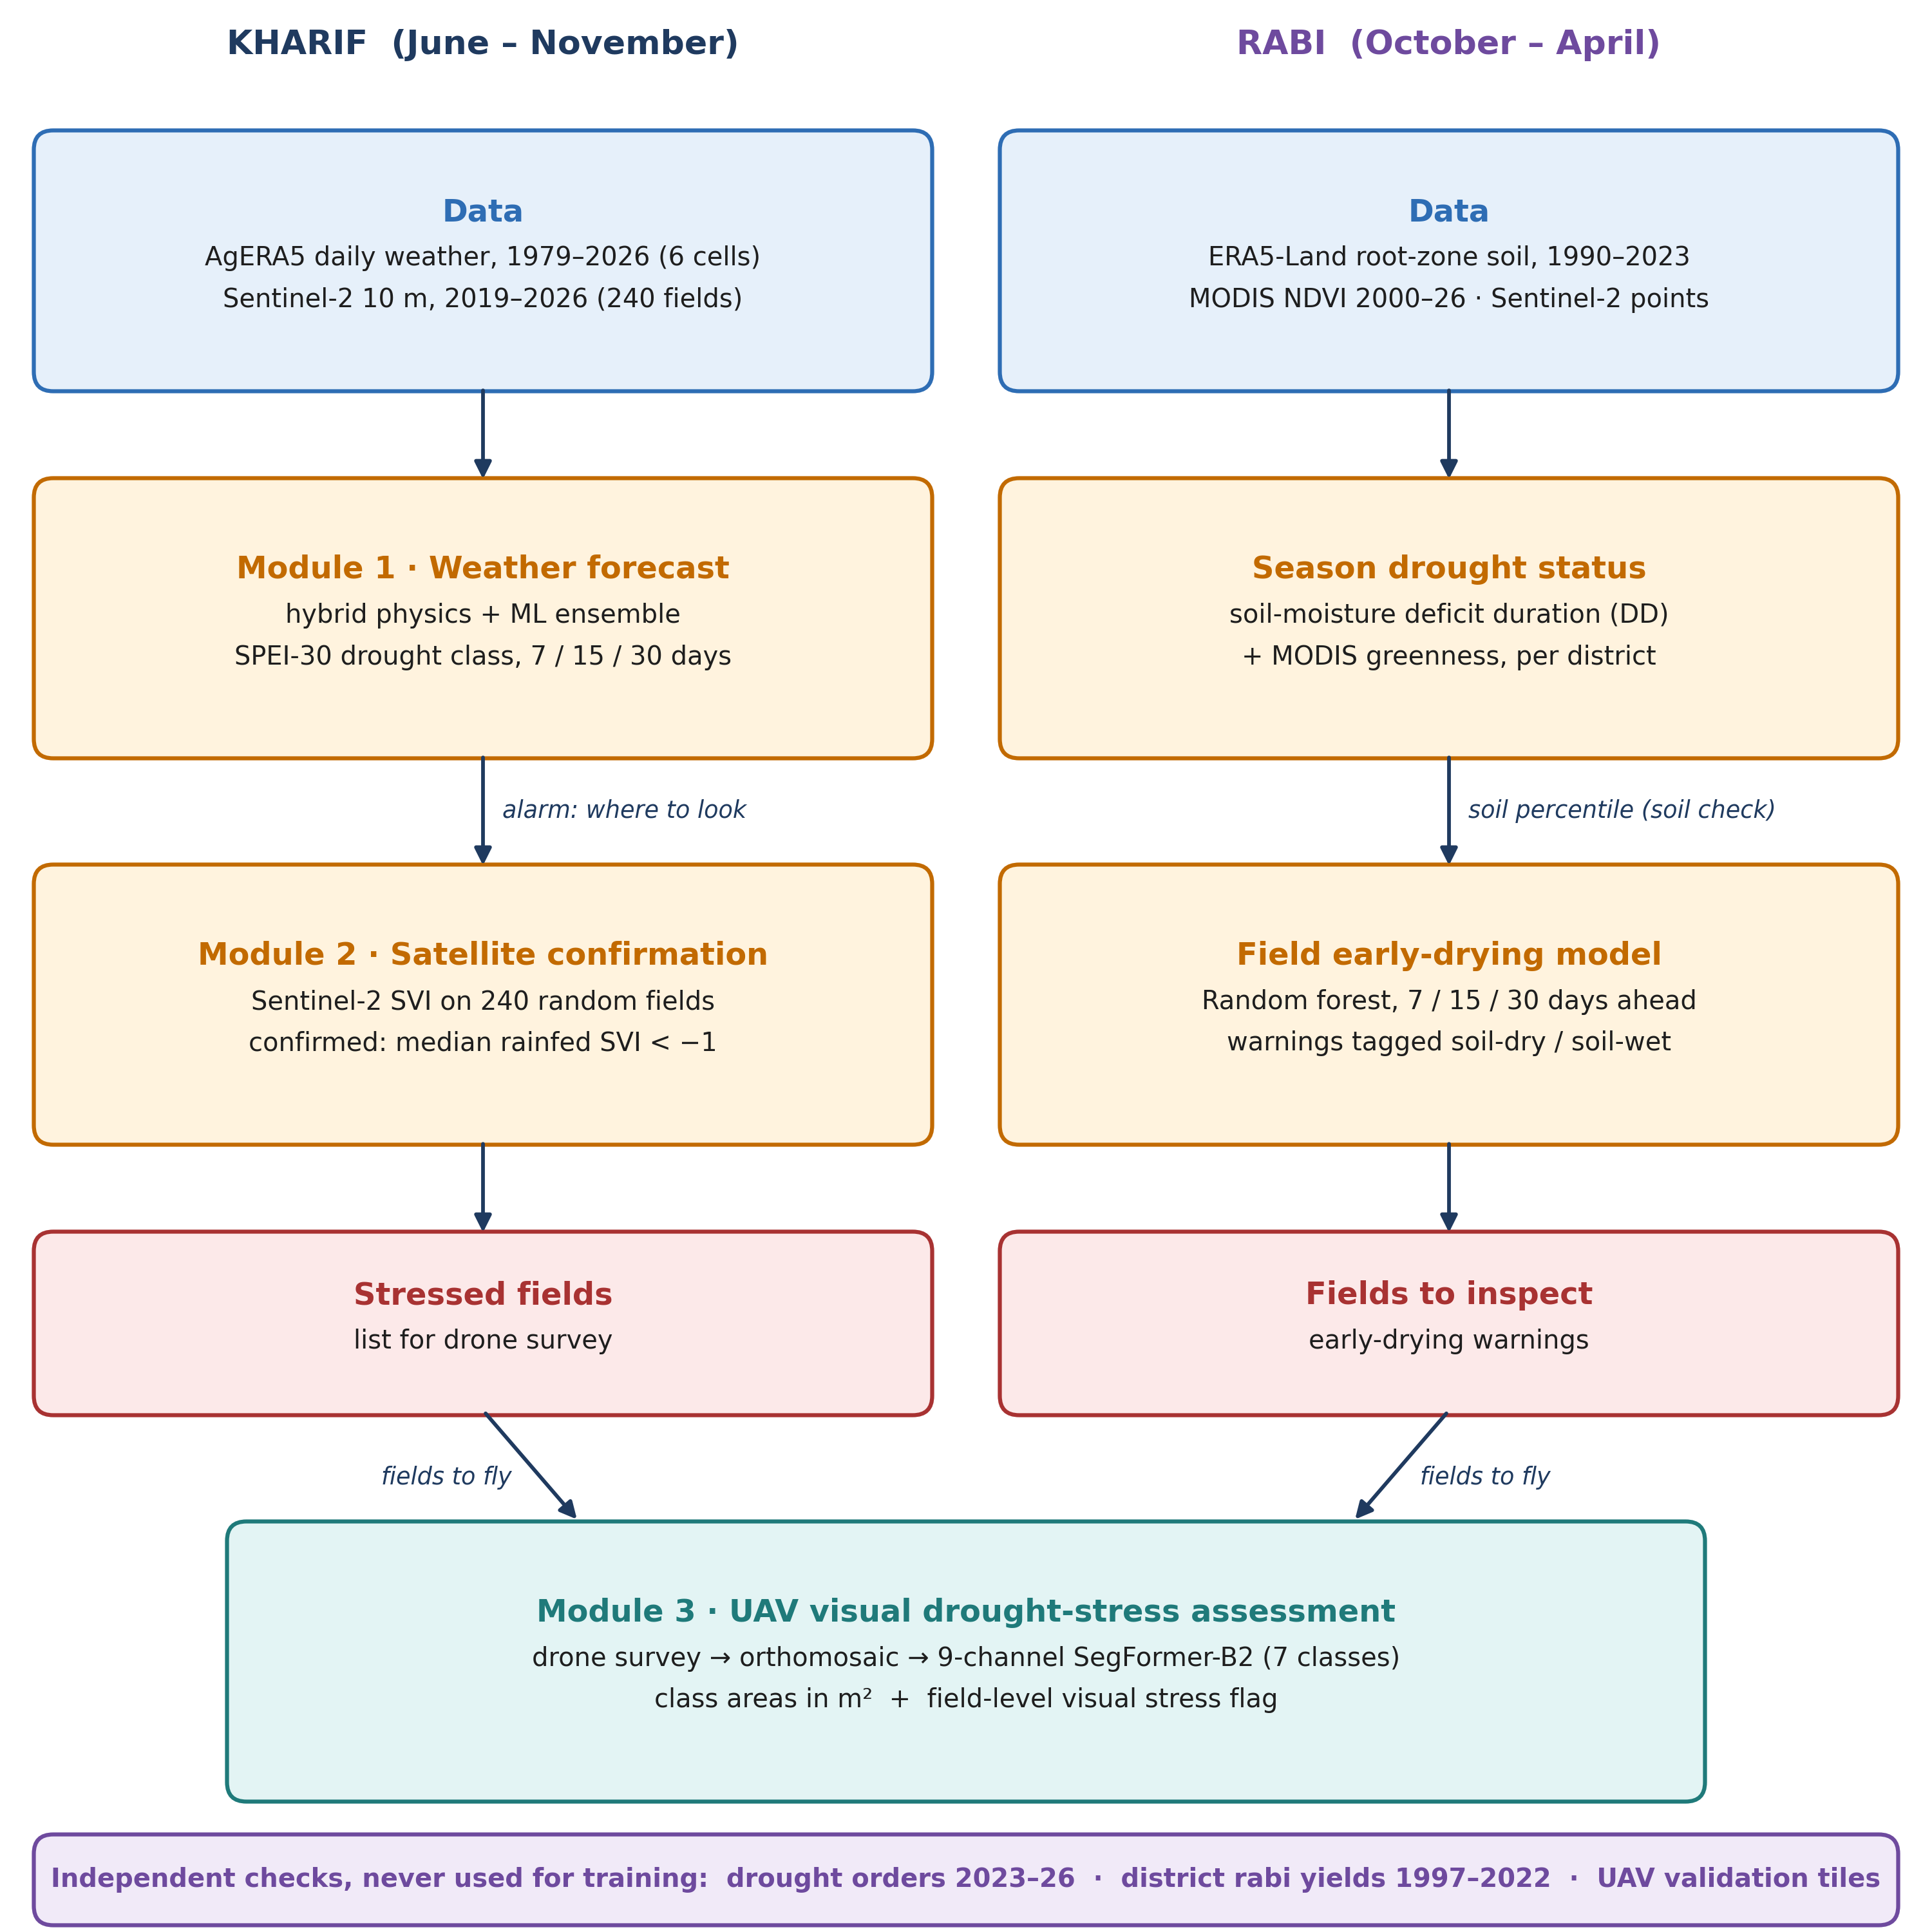
\includegraphics[height=0.70\textheight]{figures/v2_system.png}\\[1mm]
{\scriptsize Kharif writes \texttt{fields\_to\_fly.csv/.kml}; rabi writes \texttt{inspection\_candidates.csv};\\ both lists go to the UAV module.}
\end{columns}
\end{frame}

% ============================================================ 7 LIT WEATHER
\begin{frame}{5.1 Literature Review -- Weather Drought Forecasting}
\footnotesize
\renewcommand{\arraystretch}{1.45}
\begin{tabularx}{\textwidth}{@{}p{3.3cm}YYY@{}}
\toprule
\textbf{Paper} & \textbf{Contribution} & \textbf{Limitation} & \textbf{Our response} \\ \midrule
\textbf{SPEI} \newline Vicente-Serrano et al., 2010 & Standardised climatic water balance ($P - \mathrm{PET}$), log-logistic fit, multiple time scales & Usually fitted on the full record, so test years leak into the labels & Fitted on 1979--2011 only and frozen \\
\textbf{LSTM SPEI forecast} \newline Dikshit et al., 2021 & LSTM forecasts monthly SPEI better than stochastic models & Monthly scale; no operational data delay; ML-only comparison & Daily forecasts with an 8-day data delay; persistence and physics baselines \\
\textbf{Deep drought prediction} \newline Marusov et al., 2024 & Deep networks predict drought from gridded weather & Compared mainly with other ML models & Hybrid physics + ML; their protocol used as a check \\
\textbf{Wavelet ANN / SVR} \newline Belayneh et al., 2014 & Wavelet-coupled ANN and SVR forecast SPI & Only ML-vs-ML comparison & Persistence, Markov, climatology, water-balance baselines \\
\bottomrule
\end{tabularx}
\begin{block}{Our direction}
\footnotesize 30-day window of daily weather + SPEI history + \textbf{water-balance physics} $\rightarrow$ drought class 7 / 15 / 30 days ahead, with leakage-free chronological testing.
\end{block}
\end{frame}

% ============================================================ 8 WEATHER METHOD
\begin{frame}{5.2 Weather Module -- Method}
\begin{columns}[T]
\column{0.43\textwidth}
\begin{block}{Labels: SPEI-30 drought class}
\footnotesize
$D_t = P_t - \mathrm{ET}_{0,t}$, \quad $\mathrm{WB30}_t = \sum_{k=0}^{29} D_{t-k}$\\[2pt]
$\mathrm{SPEI} = \Phi^{-1}\!\big(F(\mathrm{WB30})\big)$, log-logistic fitted per site and month on \textbf{1979--2011} only, then frozen.\\[2pt]
Healthy $\ge 0$ \;$\cdot$\; Moderate $-1.5$ to $0$ \;$\cdot$\; Severe $< -1.5$
\end{block}
\begin{block}{Inputs and models}
\footnotesize
\begin{itemize}
\item 30-day window: 9 weather variables, SPEI history, day of year
\item \textbf{Water-balance ensemble}: fill the unknown future days with each 1979--2011 year $\rightarrow$ class probabilities $\hat p_c$
\item RF, XGBoost, LSTM, Transformer (5 seeds) $\rightarrow$ soft voting
\item Split: train 1979--2011, val 2012--18, test 2019--26 (purged)
\end{itemize}
\end{block}
\column{0.55\textwidth}
\centering
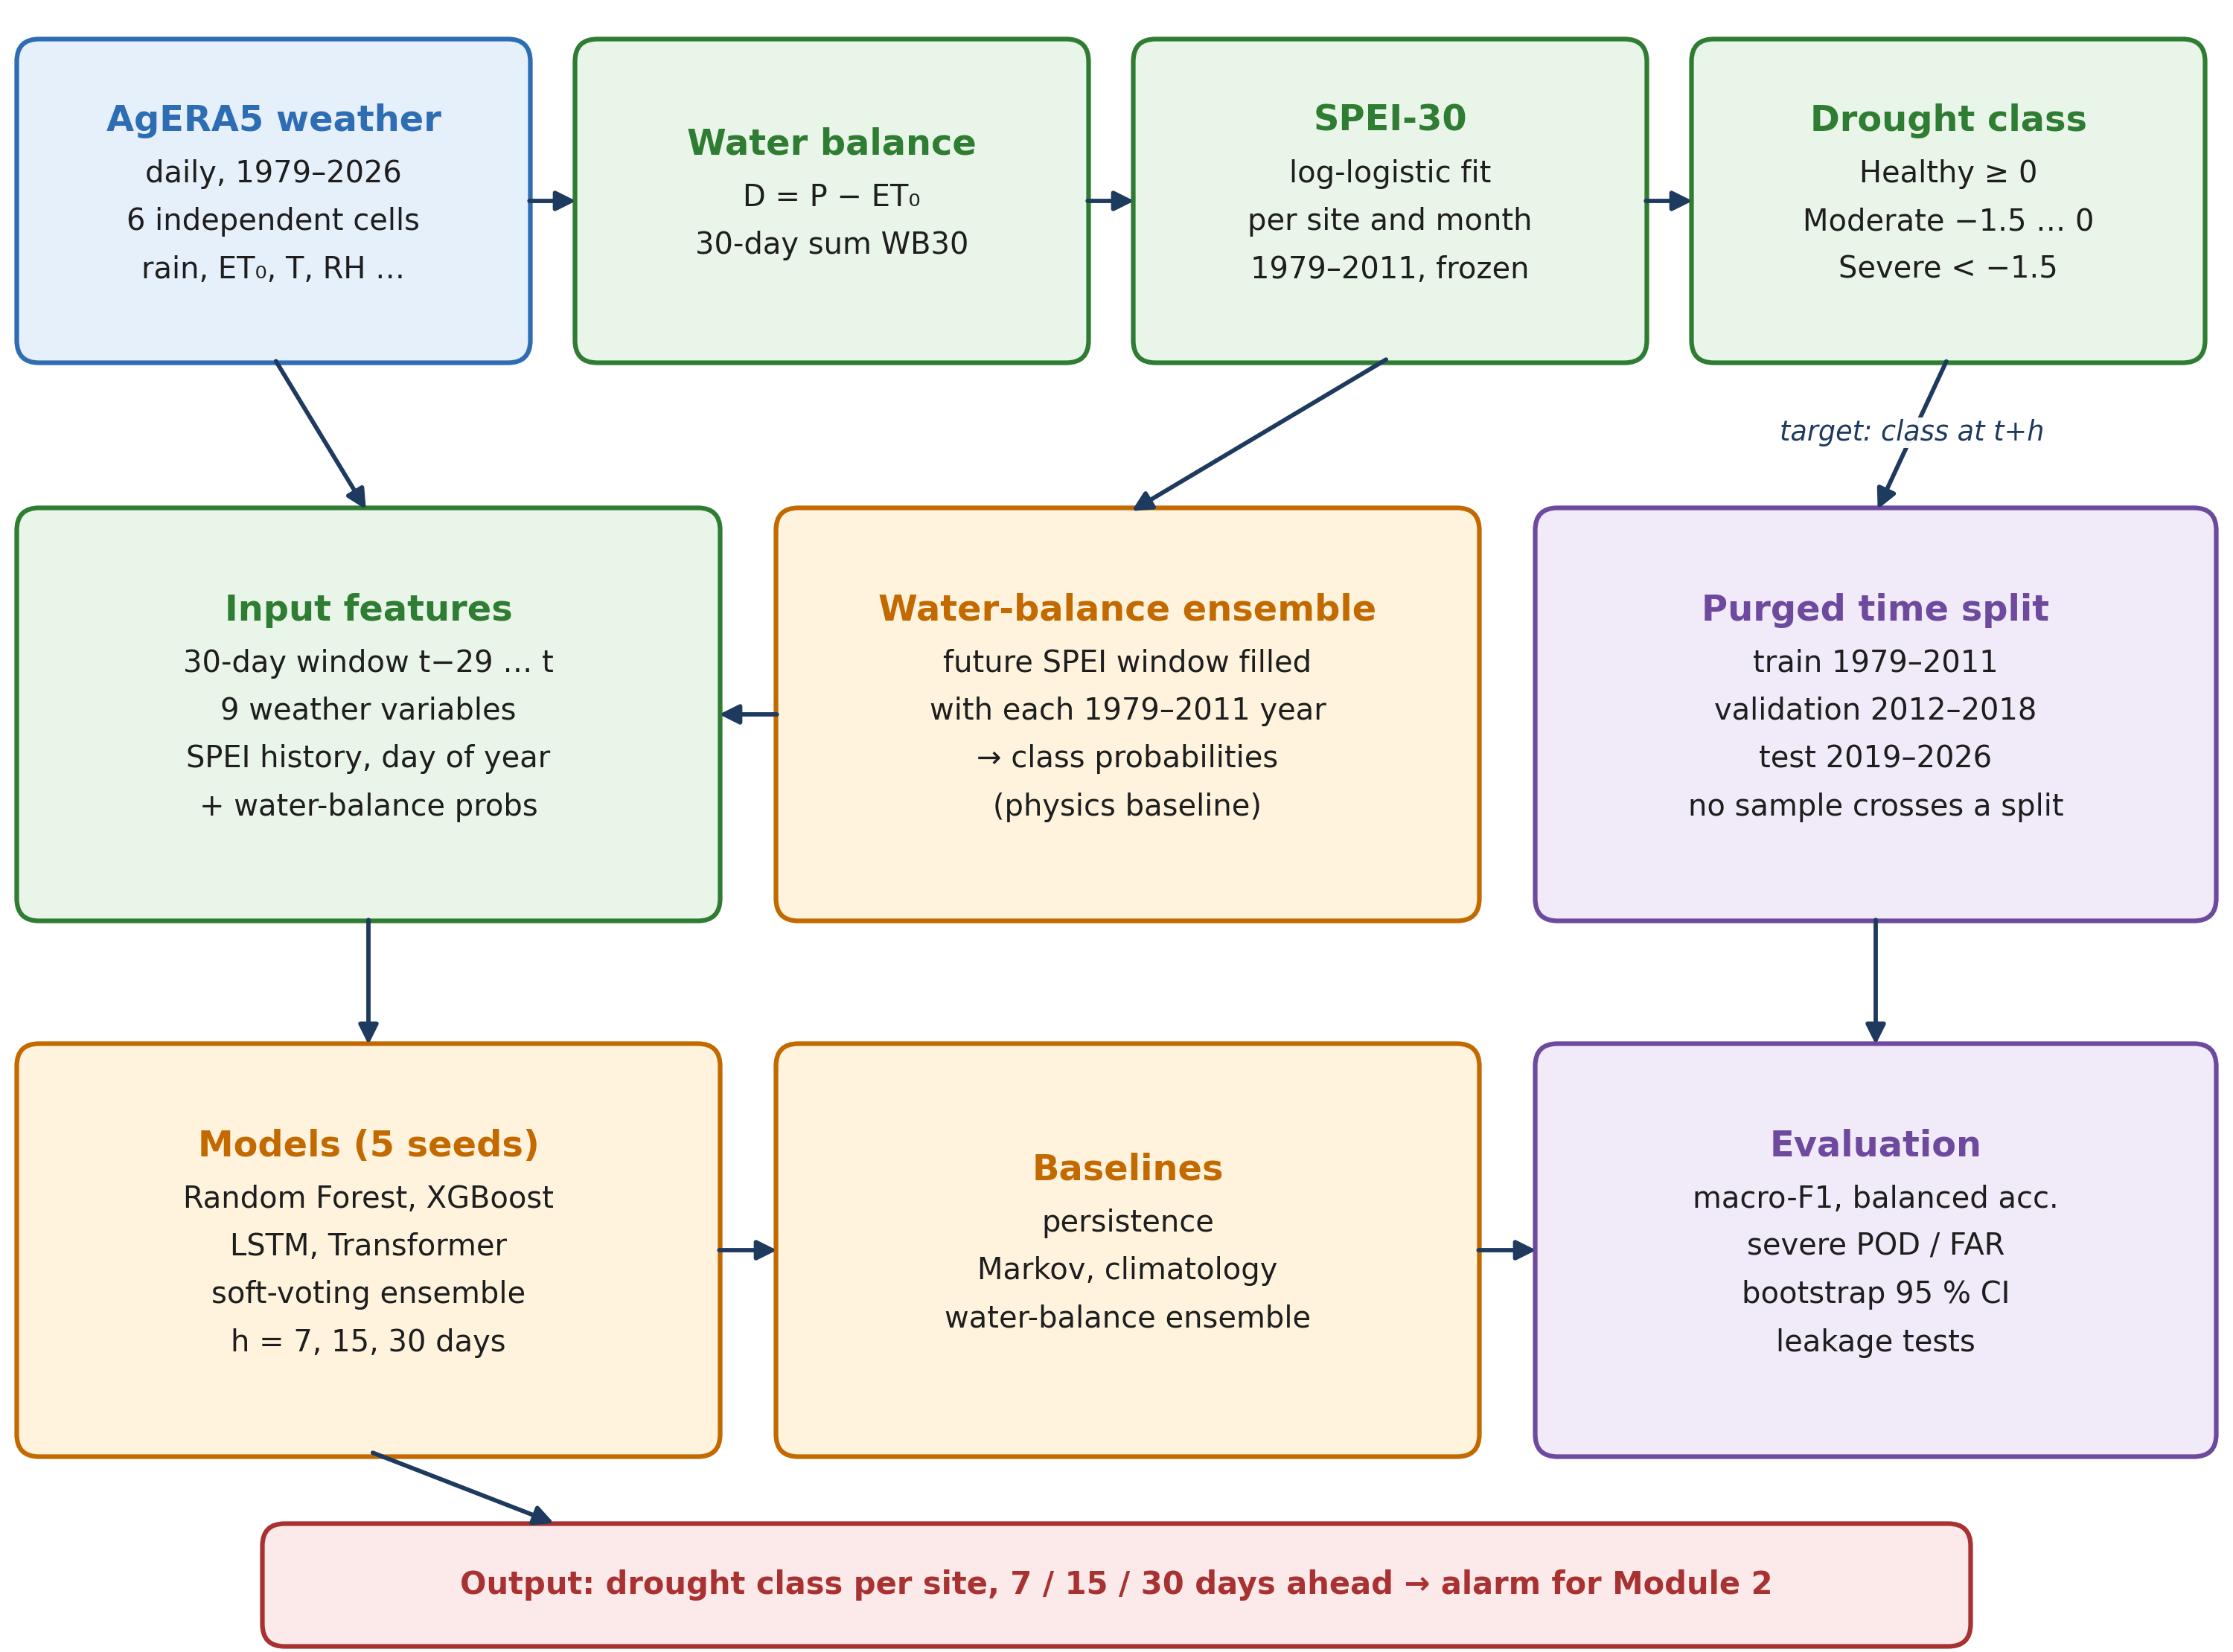
\includegraphics[width=\linewidth]{figures/v2_weather.png}
\end{columns}
\end{frame}

% ============================================================ 9 WEATHER RESULTS
\begin{frame}{5.3 Weather Module -- Results (test years 2019--2026)}
\begin{columns}[T]
\column{0.56\textwidth}
\scriptsize
\renewcommand{\arraystretch}{1.1}
\resizebox{\linewidth}{!}{%
\begin{tabular}{@{}lccc@{}}
\toprule
\textbf{Macro-F1} & \textbf{7 days} & \textbf{15 days} & \textbf{30 days} \\ \midrule
Persistence (class today) & 0.662 & 0.515 & 0.424 \\
Markov transition & 0.493 & 0.424 & 0.377 \\
Climatology & 0.309 & 0.310 & 0.310 \\
Water-balance ensemble (physics) & 0.783 & 0.592 & 0.375 \\ \midrule
Random Forest & 0.775 & 0.617 & 0.383 \\
XGBoost & 0.814 & 0.631 & 0.418 \\
LSTM & 0.806 & 0.642 & 0.406 \\
Transformer & 0.809 & 0.650 & 0.407 \\
\textbf{Soft-voting ensemble (hybrid)} & \textbf{0.819} & \textbf{0.651} & \textbf{0.424} \\ \midrule
Balanced accuracy / ROC-AUC & 85.6\% / 0.97 & 68.3\% / 0.90 & 42.5\% / 0.68 \\
\bottomrule
\end{tabular}}\\[3pt]
\centering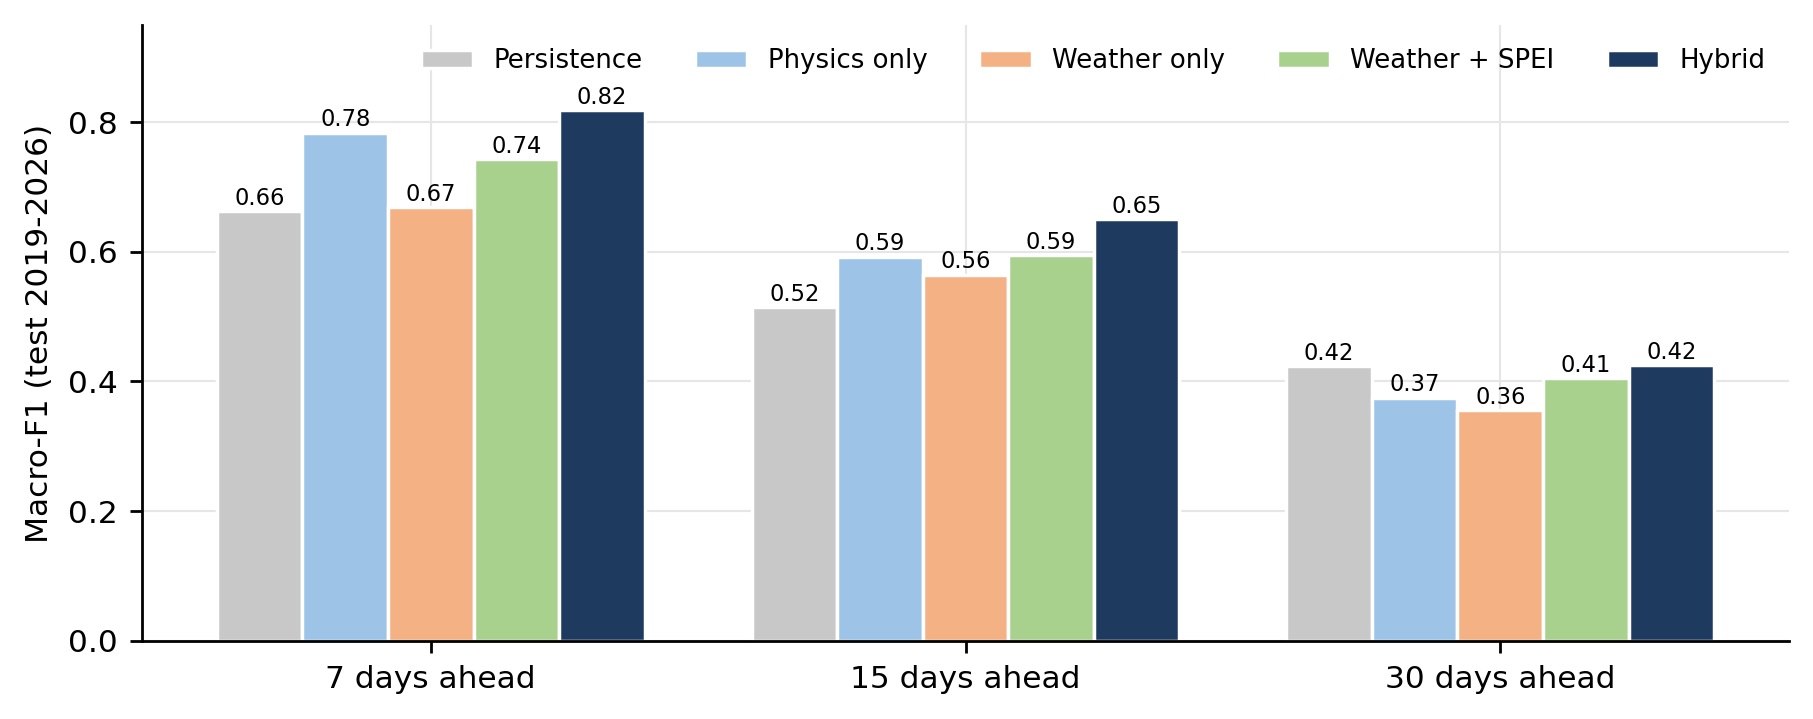
\includegraphics[width=0.72\linewidth]{figures/res_w_bars.png}
\column{0.41\textwidth}
\begin{exampleblock}{Key findings}
\footnotesize
\begin{itemize}
\item Hybrid \textbf{0.819} vs persistence 0.662 at 7 days; \textbf{0.651} vs 0.515 at 15 days.
\item Beats the physics model significantly at 15 days (95\% CI [+0.010, +0.099]).
\item Water-balance probabilities are the most valuable input (+0.063 at 7 days).
\item Severe drought: \textbf{80\%} of severe days caught 7 days ahead (false-alarm ratio 0.34).
\end{itemize}
\end{exampleblock}
\begin{alertblock}{Honest limit}
\footnotesize At 30 days no model beats persistence.
\end{alertblock}
\end{columns}
\end{frame}

% ============================================================ 10 LIT SATELLITE
\begin{frame}{5.4 Literature Review -- Satellite Drought Monitoring}
\footnotesize
\renewcommand{\arraystretch}{1.45}
\begin{tabularx}{\textwidth}{@{}p{3.3cm}YYY@{}}
\toprule
\textbf{Paper} & \textbf{Contribution} & \textbf{Limitation} & \textbf{Our response} \\ \midrule
\textbf{VCI} \newline Kogan, 1995 & NDVI scaled between historical minimum and maximum & Needs long records; with 4--5 years many dates get VCI $\approx 0$ by chance & VCI only as input; SVI as label \\
\textbf{SVI} \newline Peters et al., 2002 & z-score of NDVI for each date & Usually at coarse scale & Per field and day of year, scored year removed from the normal \\
\textbf{ML index blending} \newline Park et al., 2016 & RF / boosting on 16 MODIS + TRMM drought factors & Coarse; index-vs-index validation & 10\,m fields validated against government orders \\
\textbf{Sentinel-2 + ML, India} \newline Sharma et al., 2025 & Sentinel-2 indices with RF / XGBoost for drought detection & District ground truth; no forecasting & Chronological forecast and live replay with data delays \\
\bottomrule
\end{tabularx}
\begin{block}{Our direction}
\footnotesize 240 randomly sampled fields $\rightarrow$ Sentinel-2 SVI $\rightarrow$ lag to weather, crop-condition forecast, and replay against drought G.O.s.
\end{block}
\end{frame}

% ============================================================ 11 SATELLITE
\begin{frame}{5.5 Satellite Module -- Method and Results}
\begin{columns}[T]
\column{0.45\textwidth}
\begin{block}{Fields and label}
\footnotesize
\begin{itemize}
\item Farmland within 3\,km of each site mapped in Earth Engine; SNIC field segments (0.3--10\,ha)
\item Seeded random sample: \textbf{240 fields} (20 rainfed + 10 irrigated per site)
\item $\mathrm{SVI}_{f,d} = (\mathrm{NDVI}_{f,d} - \mu_{f,\mathrm{doy}}) / \sigma_{f,\mathrm{doy}}$, normals to 2023 with the scored year removed
\end{itemize}
\end{block}
\begin{exampleblock}{Results}
\scriptsize
\renewcommand{\arraystretch}{1.15}
\begin{tabular}{@{}lcc@{}}
\toprule
\textbf{Lag (SVI vs SPEI)} & \textbf{2019--23} & \textbf{2024--26} \\ \midrule
Rainfed: SPEI-30, 10 days & $\rho$ 0.48 & 0.45 \\
Irrigated: SPEI-60, 15 days & 0.24 & 0.29 \\ \midrule
\textbf{15-day forecast} & \textbf{RF} & \textbf{Persist.} \\ \midrule
Macro-F1 (SVI class) & \textbf{0.68} & 0.65 \\
Onset AUC (logistic 0.72) & \textbf{0.76} & 0.50 \\
\bottomrule
\end{tabular}\\[2pt]
Crops respond about \textbf{10 days} after weather drought.
\end{exampleblock}
\column{0.53\textwidth}
\centering
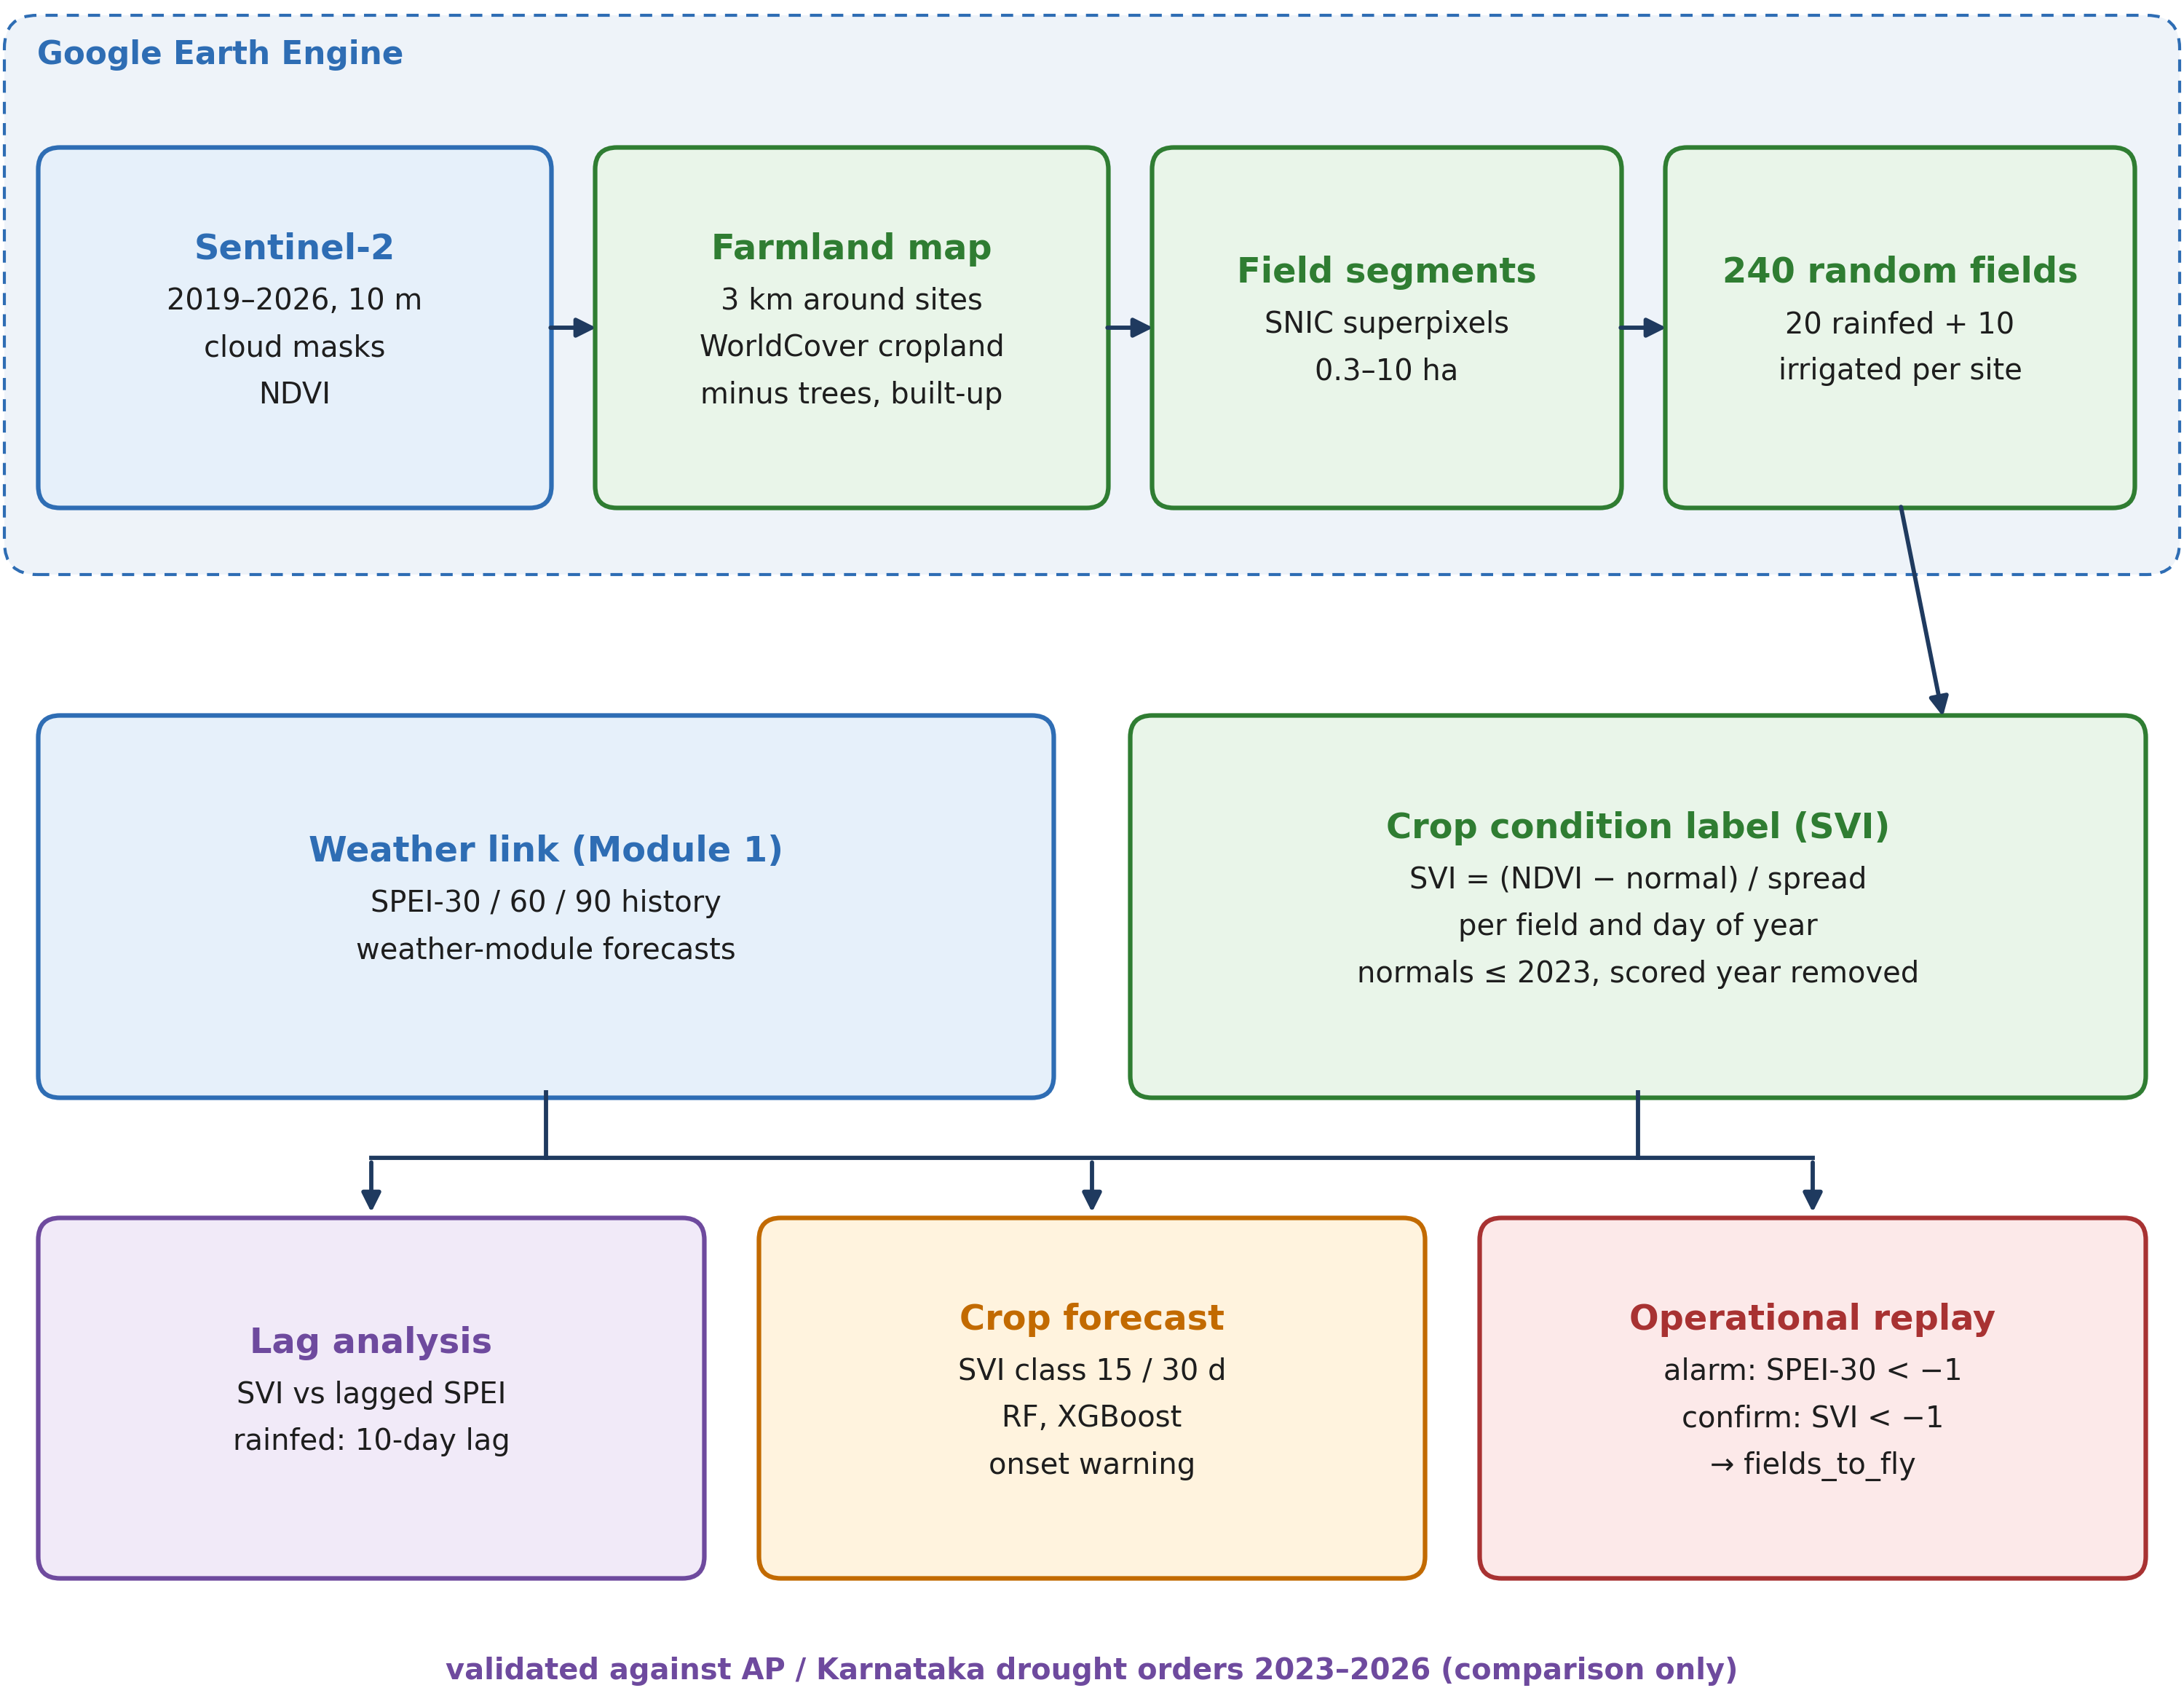
\includegraphics[width=\linewidth]{figures/v2_satellite.png}
\end{columns}
\end{frame}

% ============================================================ 12 REPLAY
\begin{frame}{5.6 Kharif Chain -- Replay against Government Drought Orders}
\begin{columns}[T]
\column{0.44\textwidth}
\begin{block}{Rules (no retraining, real data delays)}
\footnotesize
\begin{itemize}
\item Issued every 5 days, June--November, 2023--2026
\item Weather 7 days late, satellite 2 days late
\item \textbf{Alarm}: SPEI-30 $< -1$ or severe 15-day forecast
\item \textbf{Confirmed}: median rainfed SVI $< -1$ ($\ge 5$ clear fields)
\end{itemize}
\end{block}
\begin{exampleblock}{Results}
\scriptsize
\renewcommand{\arraystretch}{1.15}
\begin{tabular}{@{}lccc@{}}
\toprule
\textbf{Official} & \textbf{Confirmed} & \textbf{Before order} & \textbf{Mandal} \\ \midrule
Severe & \textbf{9 / 9} & 5 / 9 & 6 / 6 \\
Moderate & 3 / 6 & 3 / 6 & 2 / 4 \\
Not declared & 1 / 11 false alarm & & 1 / 8 \\
\bottomrule
\end{tabular}\\[2pt]
Two severe droughts confirmed \textbf{22 days before} the order (2026). 2025 moderate orders missed: rain was above normal.
\end{exampleblock}
\column{0.54\textwidth}
\centering
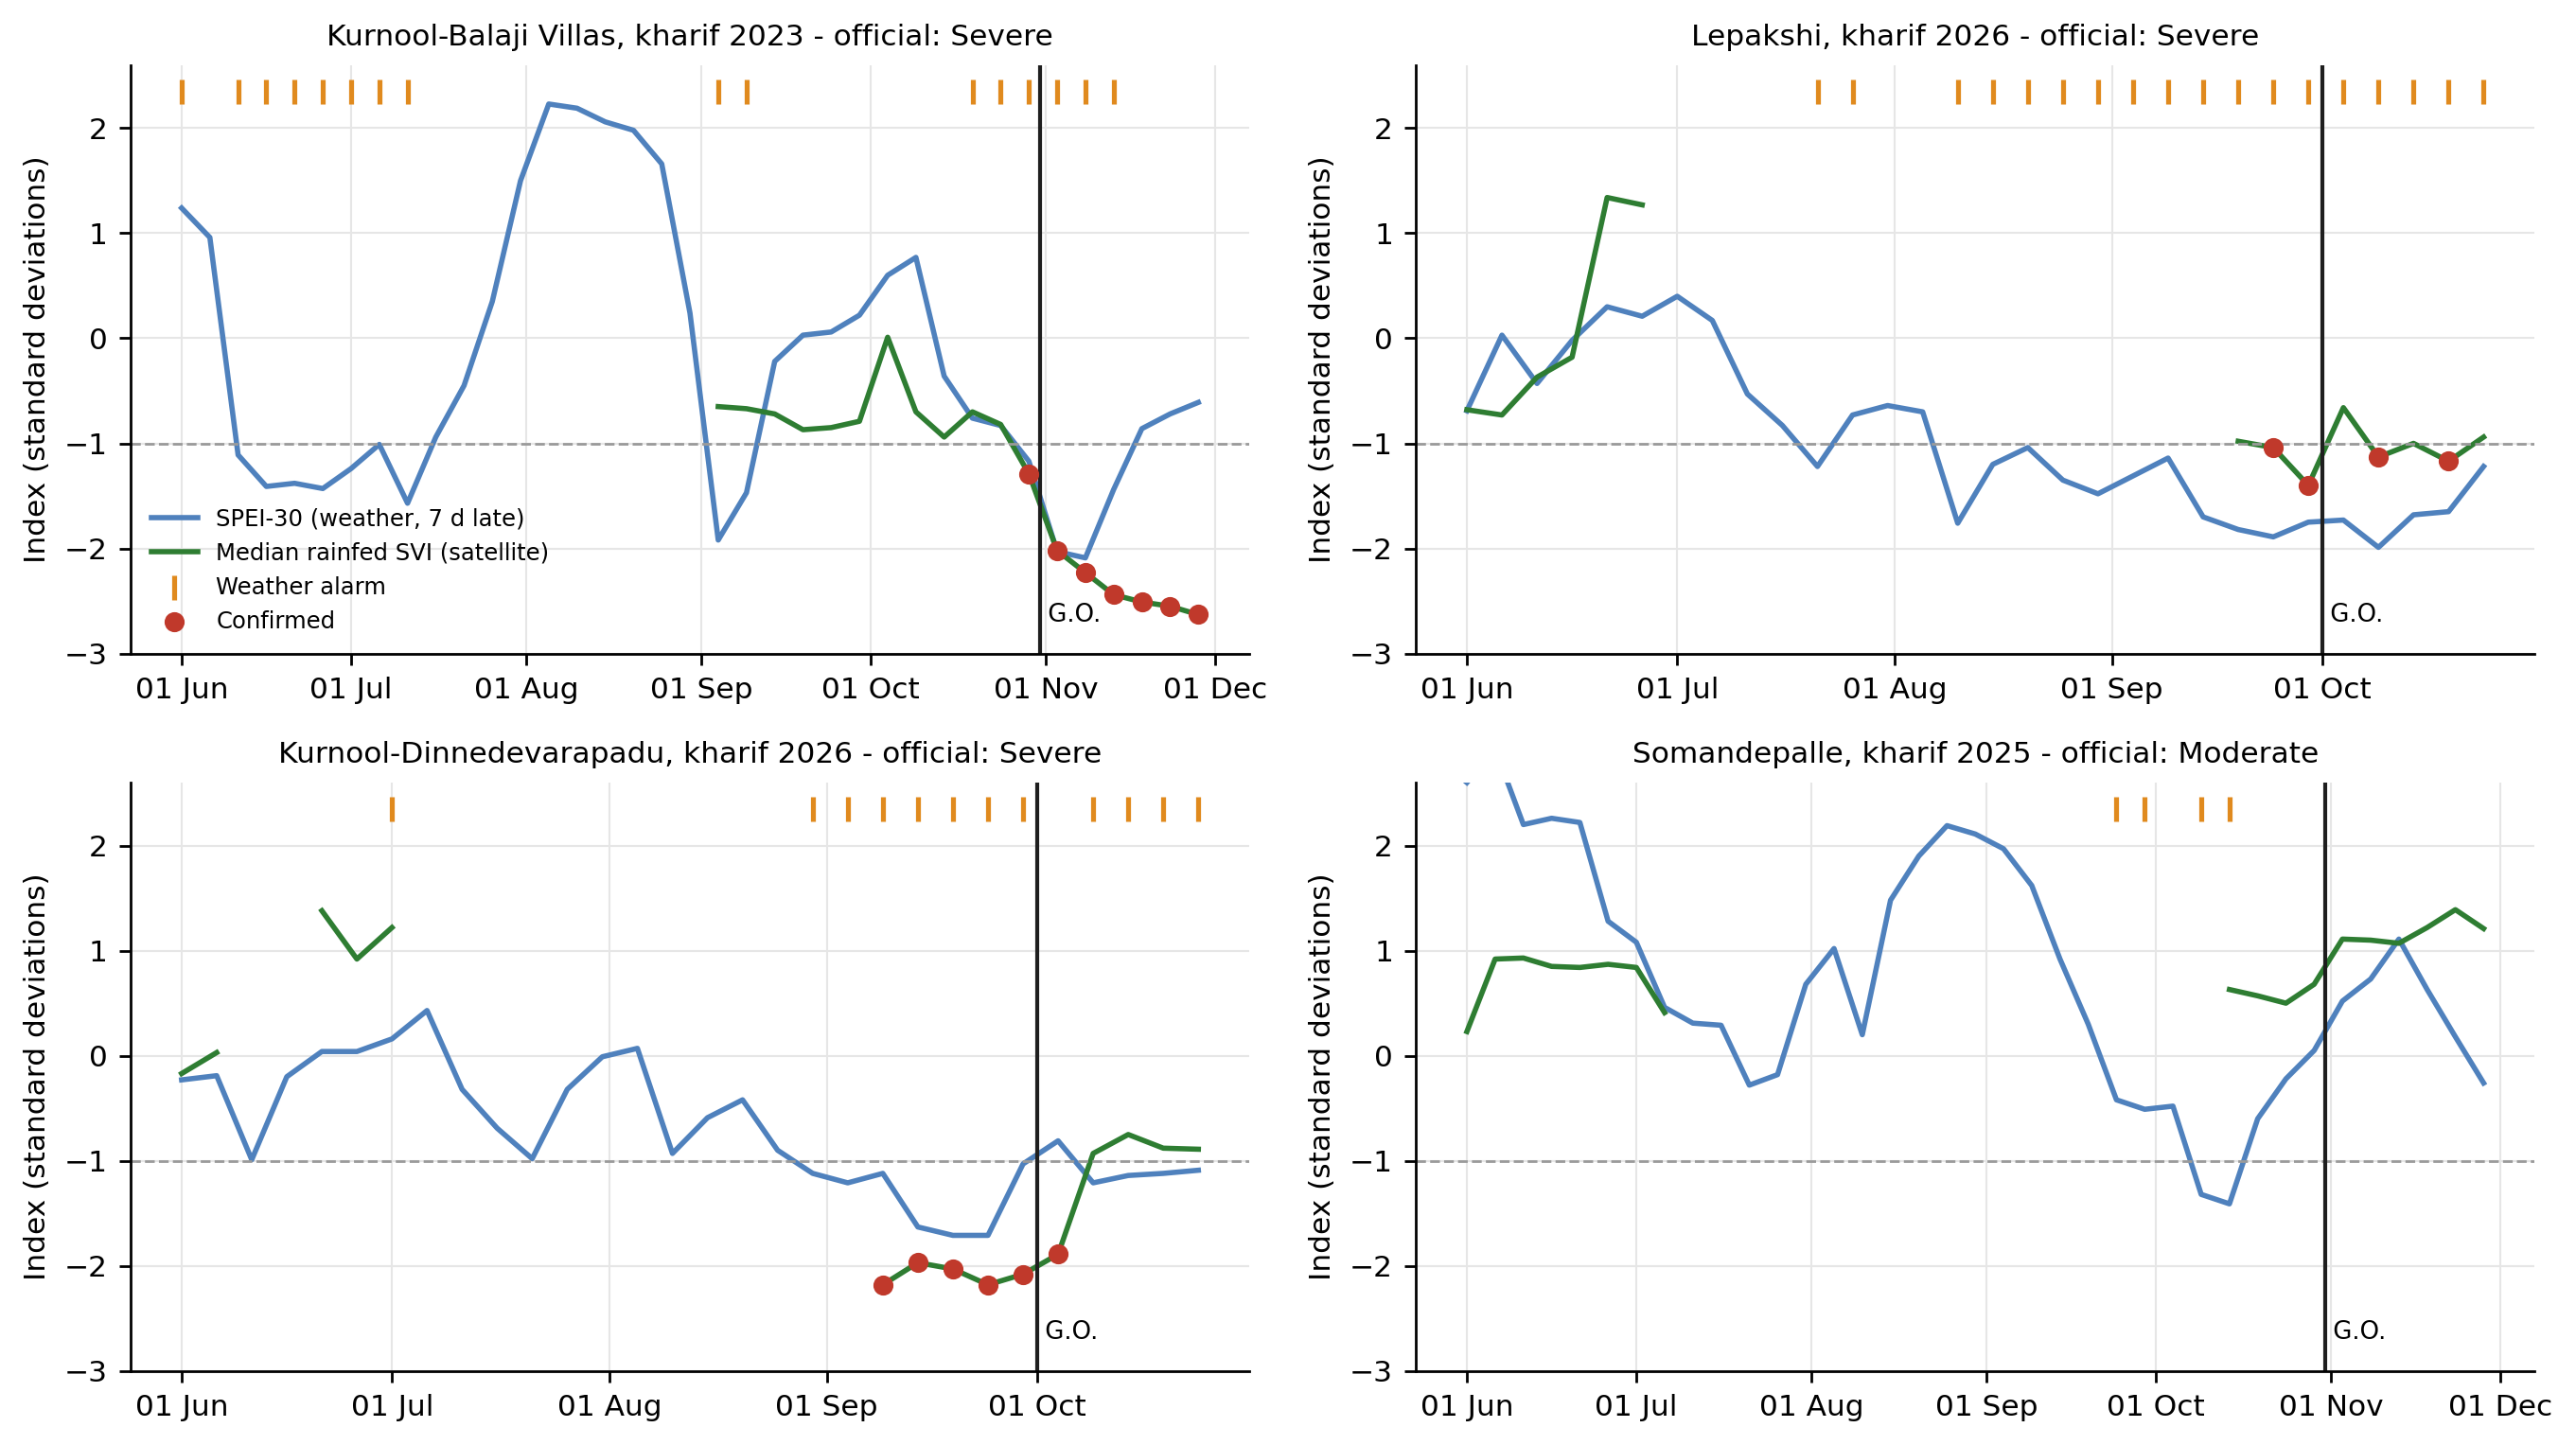
\includegraphics[width=\linewidth]{figures/res_s_cases.png}\\
{\scriptsize SPEI-30 (blue), rainfed SVI (green), alarms (orange), confirmed (red), G.O. date (black).}
\end{columns}
\end{frame}

% ============================================================ 13 WHY RABI
\begin{frame}{Why a Separate Rabi Module?}
\begin{columns}[T]
\column{0.49\textwidth}
\begin{alertblock}{1. Different water source}
\footnotesize Rabi crops (Oct--Apr) grow on soil water stored after the monsoon, irrigation and little rain, and often fail late. In-season rain is unrelated to rabi yields ($\rho = +0.01$).
\end{alertblock}
\begin{alertblock}{2. The kharif chain failed in rabi}
\footnotesize Applied unchanged to rabi 2023--2026, it confirmed \textbf{none of the 4} severe rabi mandal-seasons declared by the government.
\end{alertblock}
\column{0.49\textwidth}
\begin{alertblock}{3. Too few rabi declarations}
\footnotesize Only 4 severe rabi mandal-seasons in our area: far too few to train or test a model on government orders.
\end{alertblock}
\begin{alertblock}{4. Harvest looks like drought}
\footnotesize Greenness falls at harvest (Jan--Mar) as well as in drought, so a greenness drop alone cannot be trusted.
\end{alertblock}
\end{columns}
\vspace{3mm}
\begin{exampleblock}{Our solution}
\footnotesize Measure \textbf{root-zone soil moisture}, use it to tell drought from harvest, and validate against an independent outcome: \textbf{district crop yields} (1997--2022).
\end{exampleblock}
\end{frame}

% ============================================================ 14 LIT RABI
\begin{frame}{6.1 Literature Review -- Rabi Drought}
\footnotesize
\renewcommand{\arraystretch}{1.45}
\begin{tabularx}{\textwidth}{@{}p{3.3cm}YYY@{}}
\toprule
\textbf{Paper} & \textbf{Contribution} & \textbf{Limitation} & \textbf{Our response} \\ \midrule
\textbf{EDI + remote sensing} \newline Padhee et al., 2014 & Rabi drought in Bundelkhand from rain, soil moisture and NDVI lags & Linear, regional; not validated against crop outcomes & Soil indicator validated against district crop yields \\
\textbf{Early-season drought} \newline Nikam et al., 2020 & Early agricultural drought assessment from remote sensing & Index-based only & Independent yield outcomes, early warning by 15 Dec \\
\textbf{Sentinel-2 crop failure} \newline Descals et al., 2025 & Sentinel-2 indices decline in drought-hit winter cereals & Temperate crops, field survey; harvest not separated & Soil check separates drought from harvest \\
\textbf{Terminal drought} \newline Pang et al., 2017 & Chickpea water use and yield under terminal (late) drought & Plant-level study & Season-long soil deficit duration as indicator \\
\bottomrule
\end{tabularx}
\begin{block}{Our direction}
\footnotesize Root-zone soil moisture deficit duration + MODIS greenness $\rightarrow$ crop-loss early warning; field early-drying model checked against soil.
\end{block}
\end{frame}

% ============================================================ 15 RABI METHOD
\begin{frame}{6.2 Rabi Module -- Method}
\begin{columns}[T]
\column{0.44\textwidth}
\begin{block}{Soil drought indicator}
\footnotesize
Root zone: $\theta = 0.07\,\theta_{0\text{--}7} + 0.21\,\theta_{7\text{--}28} + 0.72\,\theta_{28\text{--}100}$ (cm)\\[2pt]
7-day mean $\rightarrow$ percentile vs the same point and date ($\pm$15 days) in 1990--2004.\\[2pt]
\textbf{Deficit day}: percentile $\le 0.20$.\\
\textbf{DD} = share of 1 Nov -- 28 Feb days in deficit.
\end{block}
\begin{block}{Outcome (never used for training)}
\footnotesize
\begin{itemize}
\item Multi-crop rabi \textbf{yield index}: each crop's yield vs median of its previous 5 seasons, fixed area weights
\item \textbf{Loss season}: index $\le -15\%$
\item Early-warning inputs end 8 days before the issue date
\end{itemize}
\end{block}
\column{0.54\textwidth}
\centering
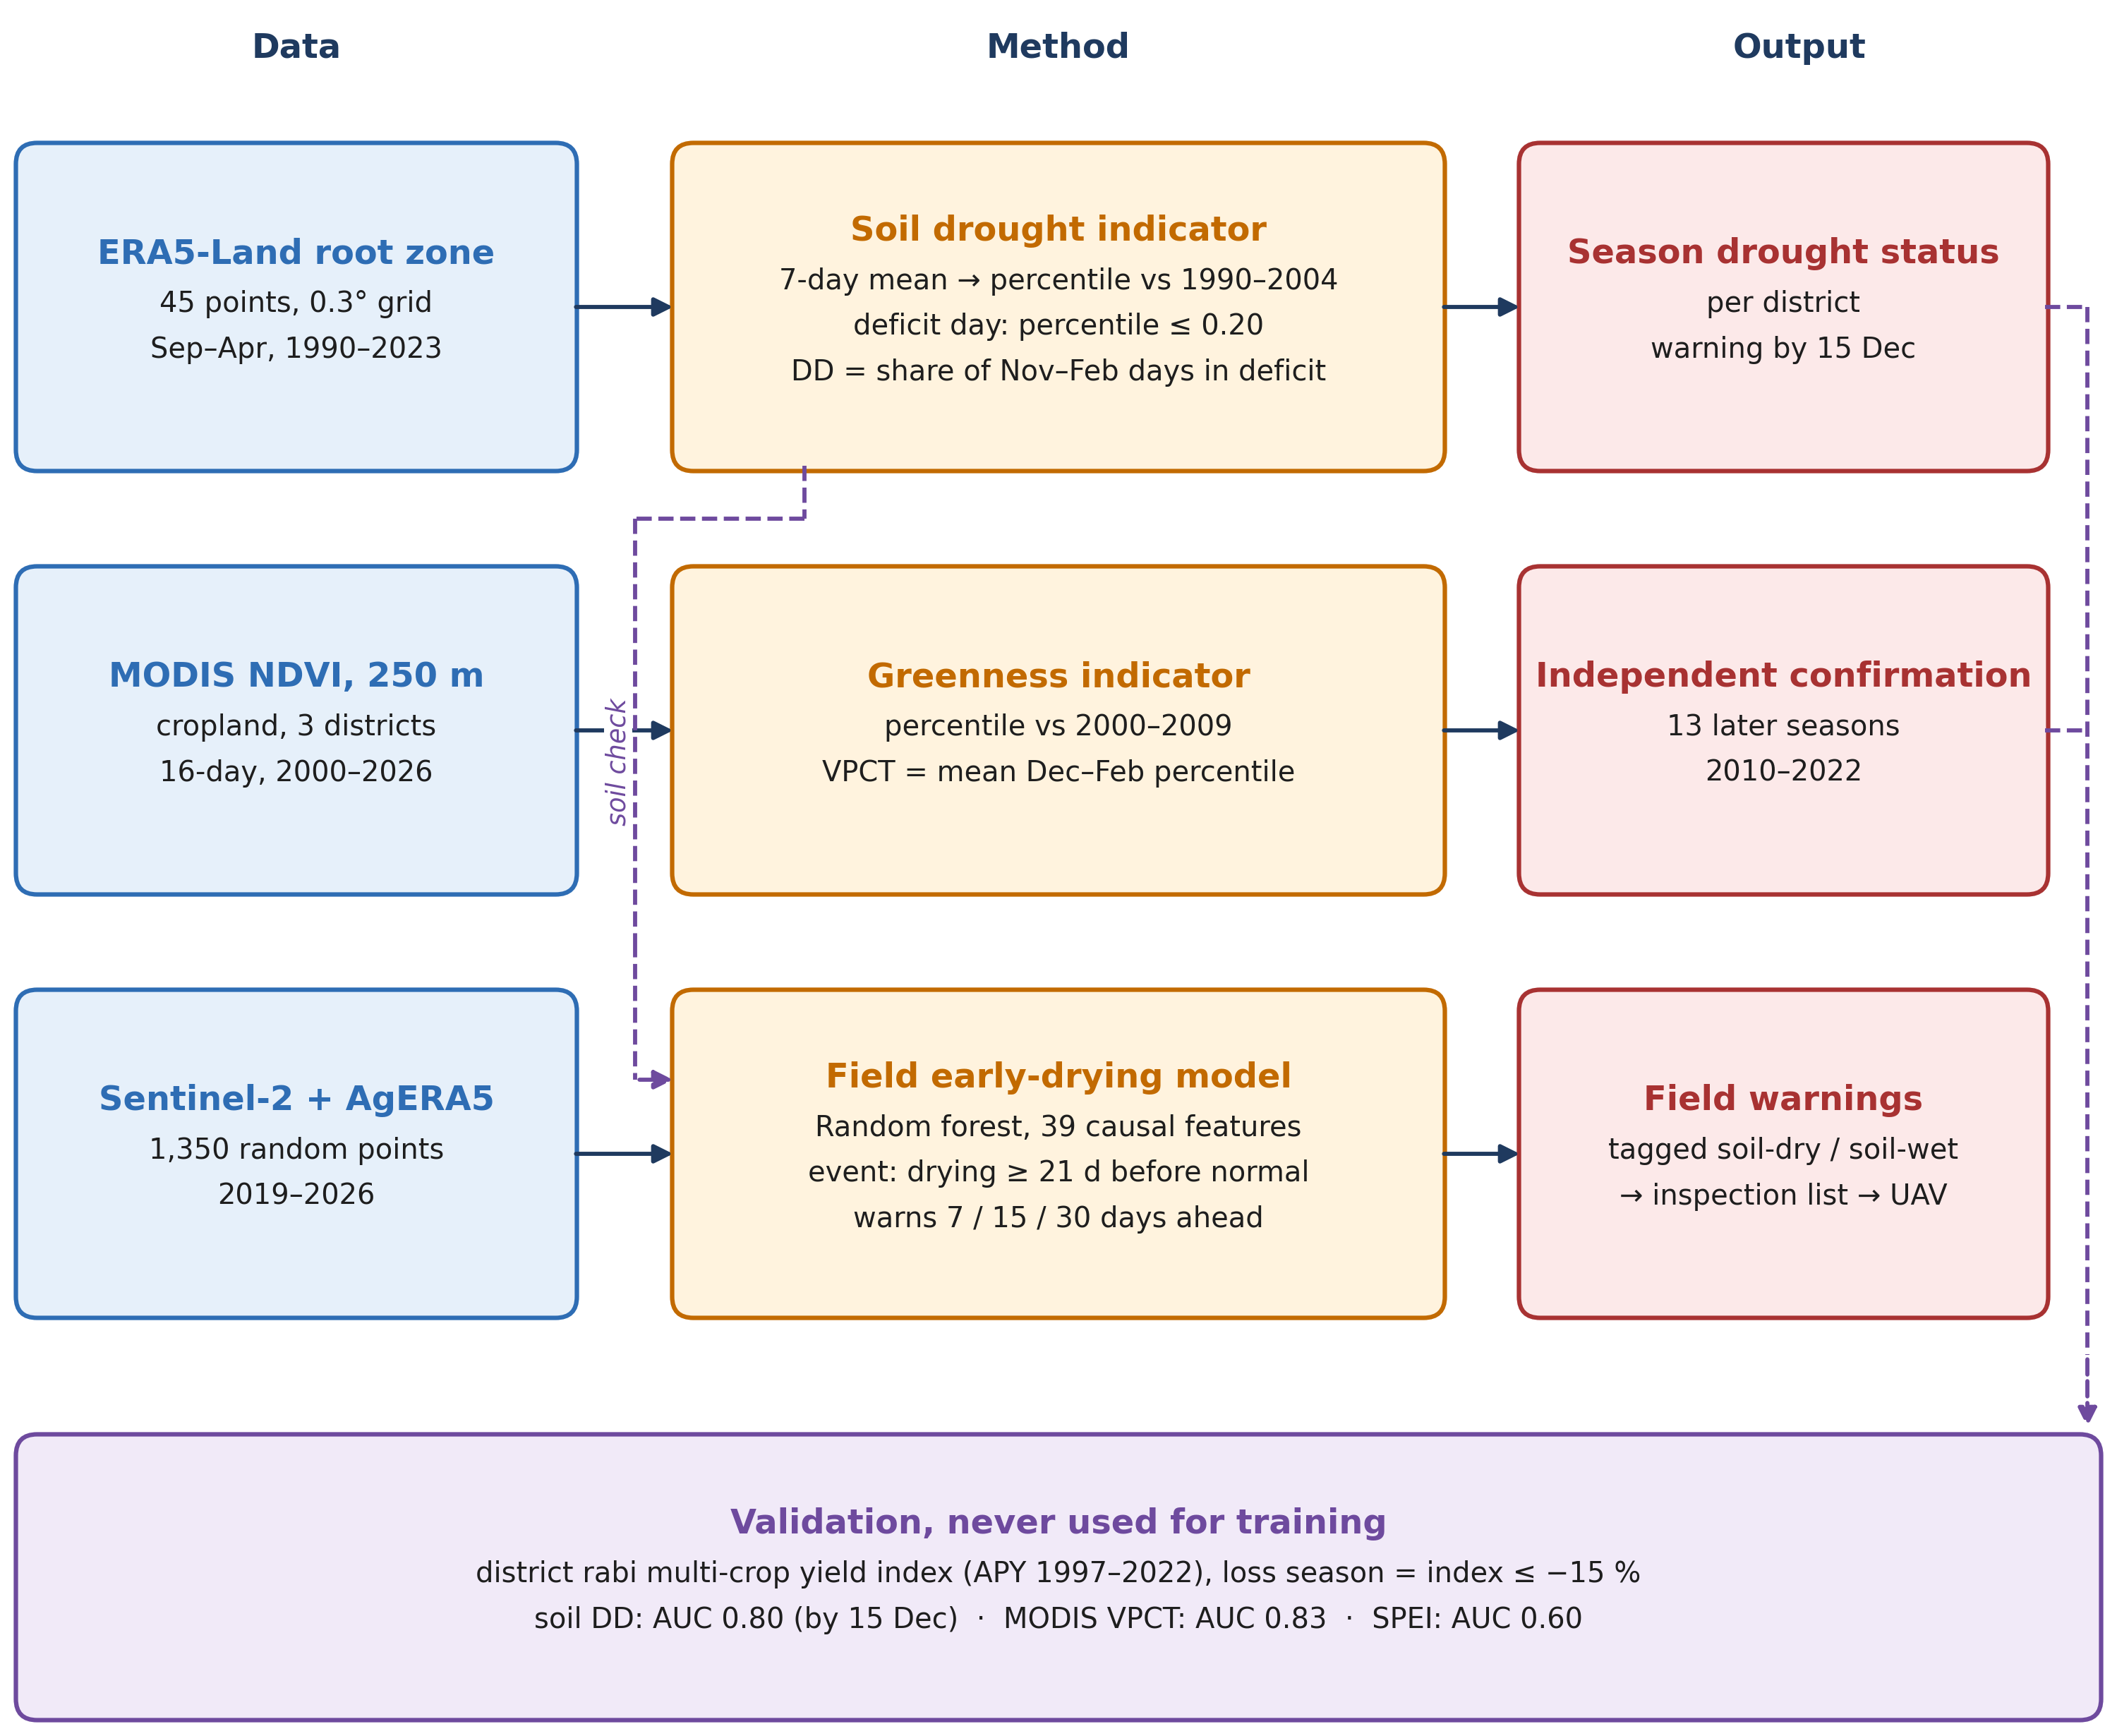
\includegraphics[width=\linewidth]{figures/v2_rabi.png}
\end{columns}
\end{frame}

% ============================================================ 16 RABI RESULTS
\begin{frame}{6.3 Rabi Module -- Results against Crop Yields}
\begin{columns}[T]
\column{0.5\textwidth}
\scriptsize
\renewcommand{\arraystretch}{1.25}
\begin{tabular}{@{}lcc@{}}
\toprule
\textbf{Indicator} (Kurnool + Anantapur) & \textbf{$\rho$ with yield} & \textbf{Loss AUC, 15 Dec} \\ \midrule
\textbf{Soil deficit duration (DD)} & $\mathbf{-0.58}$ & \textbf{0.80} \\
Soil moisture at sowing & $+0.55$ & 0.77 \\
Rain June--November & $+0.40$ & 0.72 \\
SPEI-30 & $+0.44$ & 0.60 \\
Rain Nov--Feb (in season) & $+0.01$ & -- \\
\bottomrule
\end{tabular}\\[2pt]
{\scriptsize 46 district-seasons 2000--2022, 11 loss seasons; 95\% CI by resampling seasons.}
\begin{exampleblock}{Key findings}
\footnotesize
\begin{itemize}
\item Soil deficit warns of crop-loss seasons by \textbf{15 December} (AUC 0.80) --- SPEI only 0.60.
\item \textbf{MODIS greenness} confirms on 13 independent seasons (2010--22): AUC \textbf{0.83}, $\rho$ = +0.70.
\item Two losses with wet soil and green crops are flagged by neither: losses not caused by drought.
\end{itemize}
\end{exampleblock}
\column{0.48\textwidth}
\centering
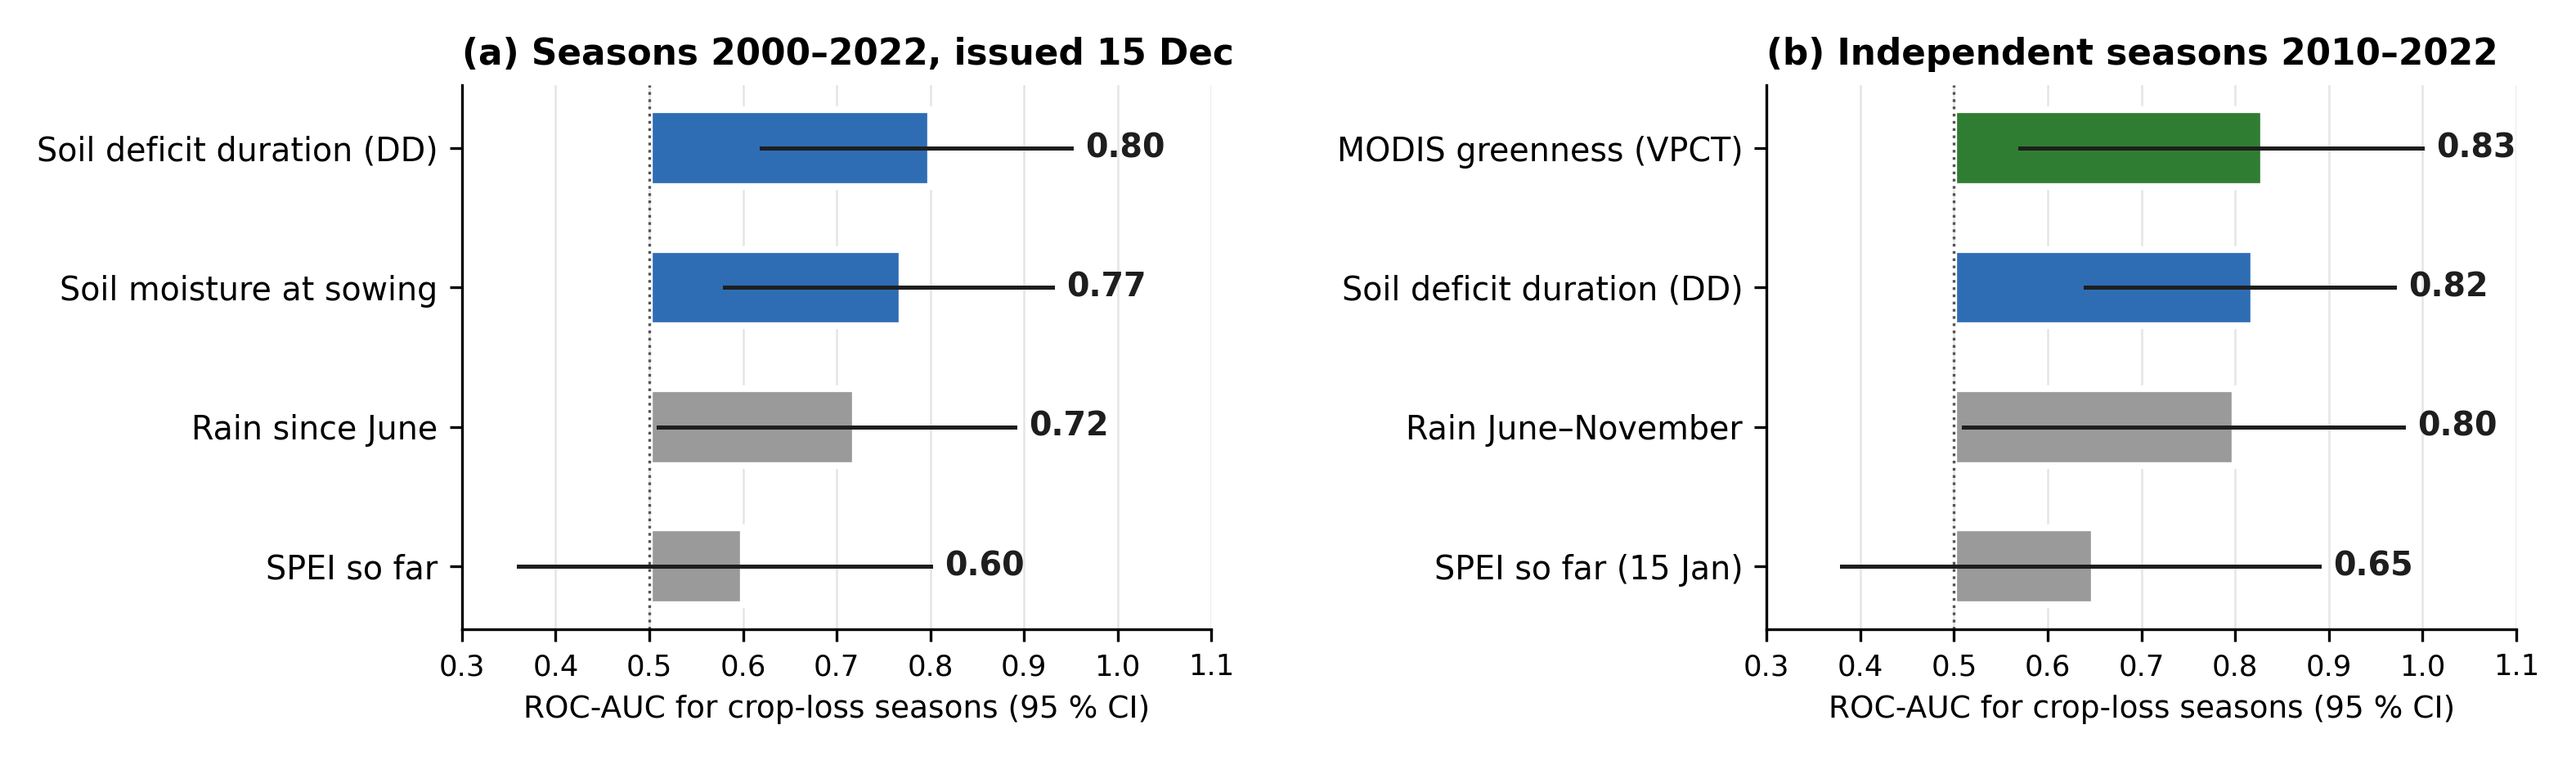
\includegraphics[width=\linewidth]{figures/rabi_auc.png}\\[2pt]
\begin{alertblock}{Limitation}
\scriptsize Districts became greener after 2010 (Dec--Feb NDVI 0.32 $\rightarrow$ 0.40), so a fixed 2000--09 greenness reference rarely flags recent seasons.
\end{alertblock}
\end{columns}
\end{frame}

% ============================================================ 17 FIELD EARLY DRYING
\begin{frame}{6.4 Rabi -- Field Early-Drying Warnings with a Soil Check}
\begin{columns}[T]
\column{0.44\textwidth}
\begin{block}{Model}
\footnotesize
\begin{itemize}
\item 1,350 random Sentinel-2 cropland points
\item \textbf{Event}: established crop dries $\ge 21$ days before the point's normal drying date
\item Random forest, 39 causal features (NDVI history, phenology, weather, root-zone soil)
\item Warns 7 / 15 / 30 days ahead; model and thresholds chosen on validation 2022 only
\item Each warning tagged \textbf{soil-dry} or \textbf{soil-wet} using the soil percentile
\end{itemize}
\end{block}
\column{0.54\textwidth}
\scriptsize
\renewcommand{\arraystretch}{1.25}
\begin{tabular}{@{}lccc@{}}
\toprule
\textbf{30 days ahead, test 2023--25} & \textbf{Precision} & \textbf{Recall} & \textbf{Lead} \\ \midrule
Validation-selected model & 0.54 & 0.28 & 16 d \\ \midrule
\multicolumn{4}{@{}l}{\textit{Same events caught (40 of 108):}} \\
Earlier model (no soil) & 0.51 & 0.37 & -- \\
Final model (39 features) & 0.56 & 0.37 & -- \\
\textbf{Final model, soil-dry warnings} & \textbf{0.69} & 0.37 & -- \\
\bottomrule
\end{tabular}
\begin{exampleblock}{Key finding}
\footnotesize Warnings under below-normal soil are correct \textbf{about twice as often} as under wet soil (0.67 vs 0.38), where greenness drops are mostly harvest.
\end{exampleblock}
\begin{alertblock}{Honest note}
\scriptsize Only 2023 had below-normal soil among the test seasons, so this contrast is descriptive. A separate 15-day NDVI forecast has 18\% lower error than the best baseline.
\end{alertblock}
\end{columns}
\end{frame}

% ============================================================ 18 LIT UAV
\begin{frame}{7.1 Literature Review -- UAV Crop Stress Segmentation}
\footnotesize
\renewcommand{\arraystretch}{1.45}
\begin{tabularx}{\textwidth}{@{}p{3.3cm}YYY@{}}
\toprule
\textbf{Paper} & \textbf{Contribution} & \textbf{Limitation} & \textbf{Our response} \\ \midrule
\textbf{SegFormer} \newline Xie et al., 2021 & Hierarchical Transformer encoder with lightweight MLP decoder & General-purpose, 3-channel RGB & 9 channels (RGB + vegetation indices), 7 crop classes \\
\textbf{Cotton water stress from UAV} \newline Shahi et al., 2023 & CNN classifies cotton water stress from UAV RGB images & Image-level classes; no area & Pixel-level segmentation and area in m$^2$ \\
\textbf{UAV weed detection} \newline Dang et al., 2023 & Compares deep segmentation networks for weeds in UAV images & Dry weeds and drought look alike & Separate dry-weed and drought classes \\
\textbf{Lov\'asz-Softmax / focal loss} \newline Berman 2018; Lin 2017 & Losses for IoU and class imbalance & -- & Combined focal + Dice + Lov\'asz loss \\
\bottomrule
\end{tabularx}
\begin{block}{Our direction}
\footnotesize 9-channel UAV orthomosaics $\rightarrow$ SegFormer-B2 $\rightarrow$ 7-class map $\rightarrow$ seam-free stitching of billion-pixel fields $\rightarrow$ area and visual stress flag.
\end{block}
\end{frame}

% ============================================================ 19 UAV DATA
\begin{frame}{7.2 UAV Data Acquisition and Photo Stitching}
\begin{columns}[T]
\column{0.34\textwidth}
\begin{block}{Flight plan}
\scriptsize
\begin{itemize}
\item DJI Mini 4 Pro (RGB camera)
\item Altitude 10--12\,m, speed 1.2--1.5\,m/s
\item Gimbal $-90^\circ$, path spacing 3--5\,m
\item Overlap 70--80\%, east--west lines
\item Flights: Nov 2025 -- Jan 2026
\end{itemize}
\centering
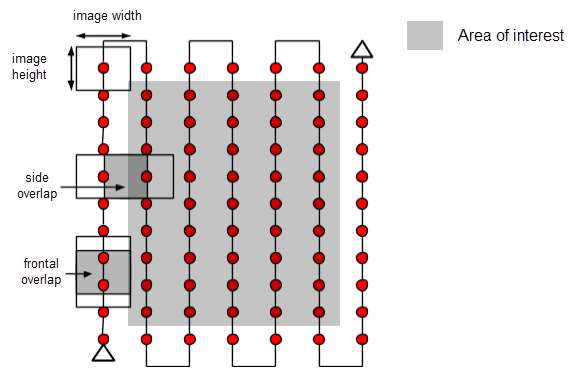
\includegraphics[width=0.72\linewidth]{figures/prof/lawnmower_path.png}\\
{\tiny Lawnmower path (source: Humboldt State Univ.)}
\end{block}
\column{0.64\textwidth}
\begin{block}{Photos $\rightarrow$ orthomosaic (Agisoft Metashape)}
\centering
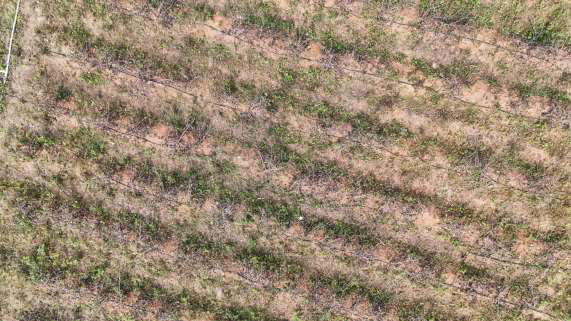
\includegraphics[height=1.75cm]{figures/prof/p11_0.png}\hspace{1mm}
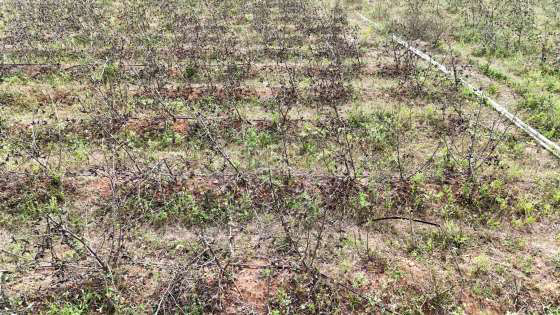
\includegraphics[height=1.75cm]{figures/prof/p11_2.png}\hspace{1mm}
{\Large$\Rightarrow$}\hspace{1mm}
\raisebox{-0.6cm}{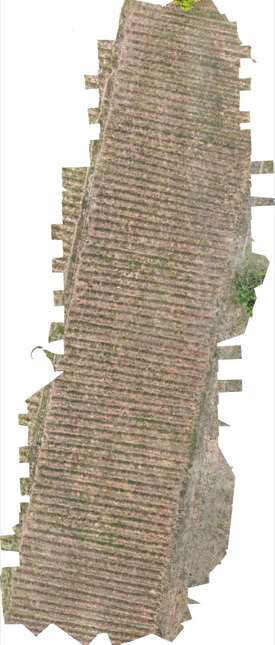
\includegraphics[height=2.4cm]{figures/prof/ortho_cotton.png}}\\[1pt]
\raggedright\scriptsize Overlapping photos are matched and aligned into one orthomosaic. \textbf{14 orthomosaics}: 3.8 million -- 2.86 billion pixels; GSD 1.68--5.55\,mm (9 fields), 3.6--18.5\,mm (5 Peddakadubur fields, low-resolution frames).
\end{block}
\centering
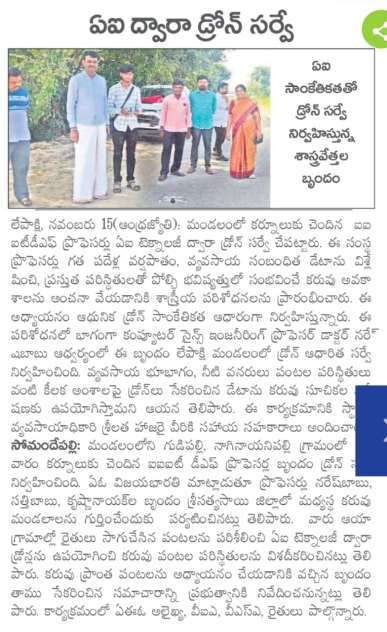
\includegraphics[height=1.95cm]{figures/prof/news_lepakshi.png}\hspace{2mm}
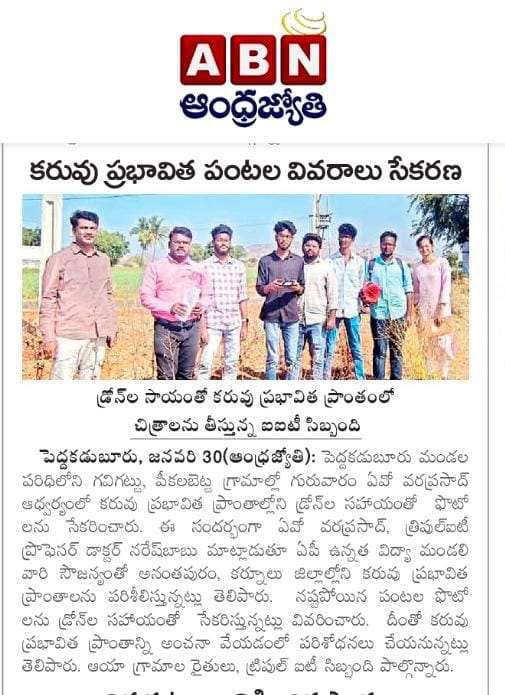
\includegraphics[height=1.95cm]{figures/prof/news_peddakadubur.png}\\
{\tiny Field surveys in Andhra Jyothy: Lepakshi (15 Nov 2025), Peddakadubur (30 Jan 2026)}
\end{columns}
\end{frame}

% ============================================================ 20 PIPELINE
\begin{frame}{7.3 UAV Module -- End-to-End Pipeline}
\begin{columns}[T]
\column{0.58\textwidth}
\centering
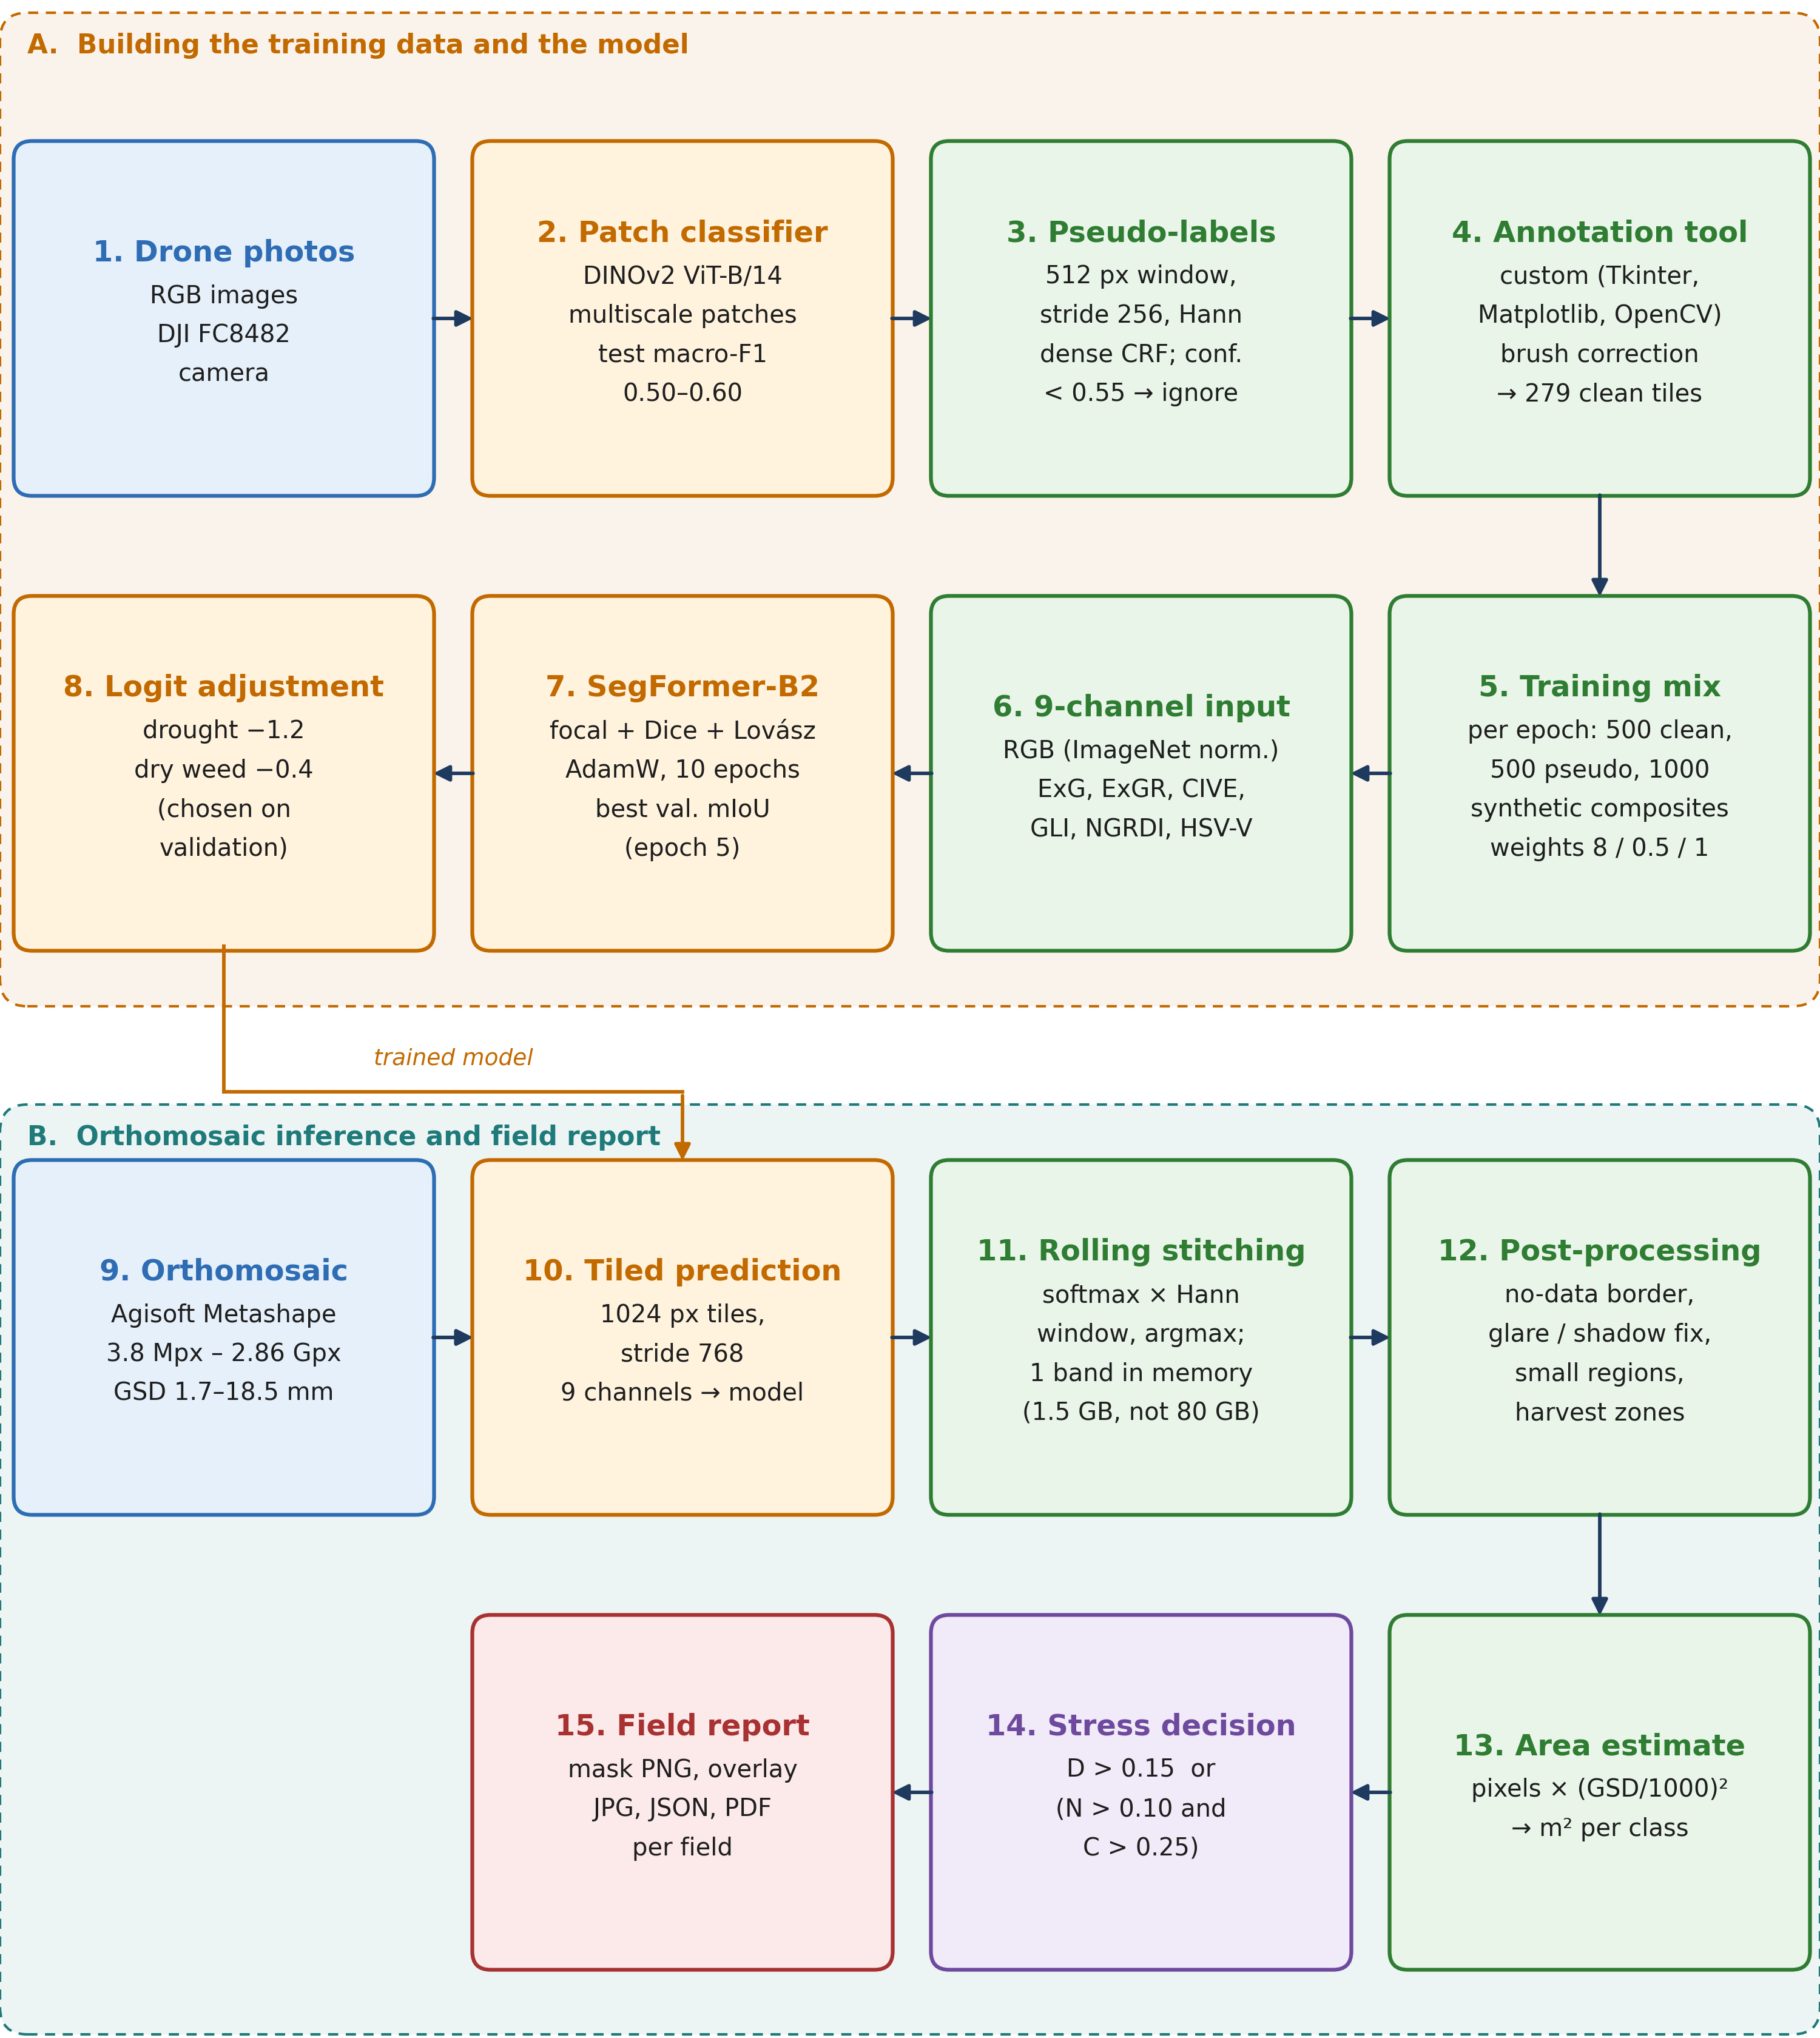
\includegraphics[height=0.86\textheight]{figures/v2_uav_pipeline.png}
\column{0.40\textwidth}
\begin{block}{Phase A -- build labels and model (1--8)}
\scriptsize Drone photos $\rightarrow$ DINOv2 patch classifier $\rightarrow$ pseudo-labels $\rightarrow$ correction in our annotation tool $\rightarrow$ training mix $\rightarrow$ 9 channels $\rightarrow$ SegFormer-B2 $\rightarrow$ logit adjustment.
\end{block}
\begin{block}{Phase B -- process one field (9--15)}
\scriptsize Orthomosaic $\rightarrow$ 1024\,px tiles $\rightarrow$ rolling Hann stitching $\rightarrow$ post-processing $\rightarrow$ area in m$^2$ $\rightarrow$ stress decision $\rightarrow$ field report (mask, overlay, JSON, PDF).
\end{block}
\begin{alertblock}{Two kinds of stitching}
\scriptsize Metashape stitches \textbf{photos} into an orthomosaic (step 9); our pipeline stitches \textbf{predictions} of overlapping tiles (step 11).
\end{alertblock}
\end{columns}
\end{frame}

% ============================================================ 21 LABELS + CHANNELS
\begin{frame}{7.4 Building Labels and the Nine Input Channels}
\centering
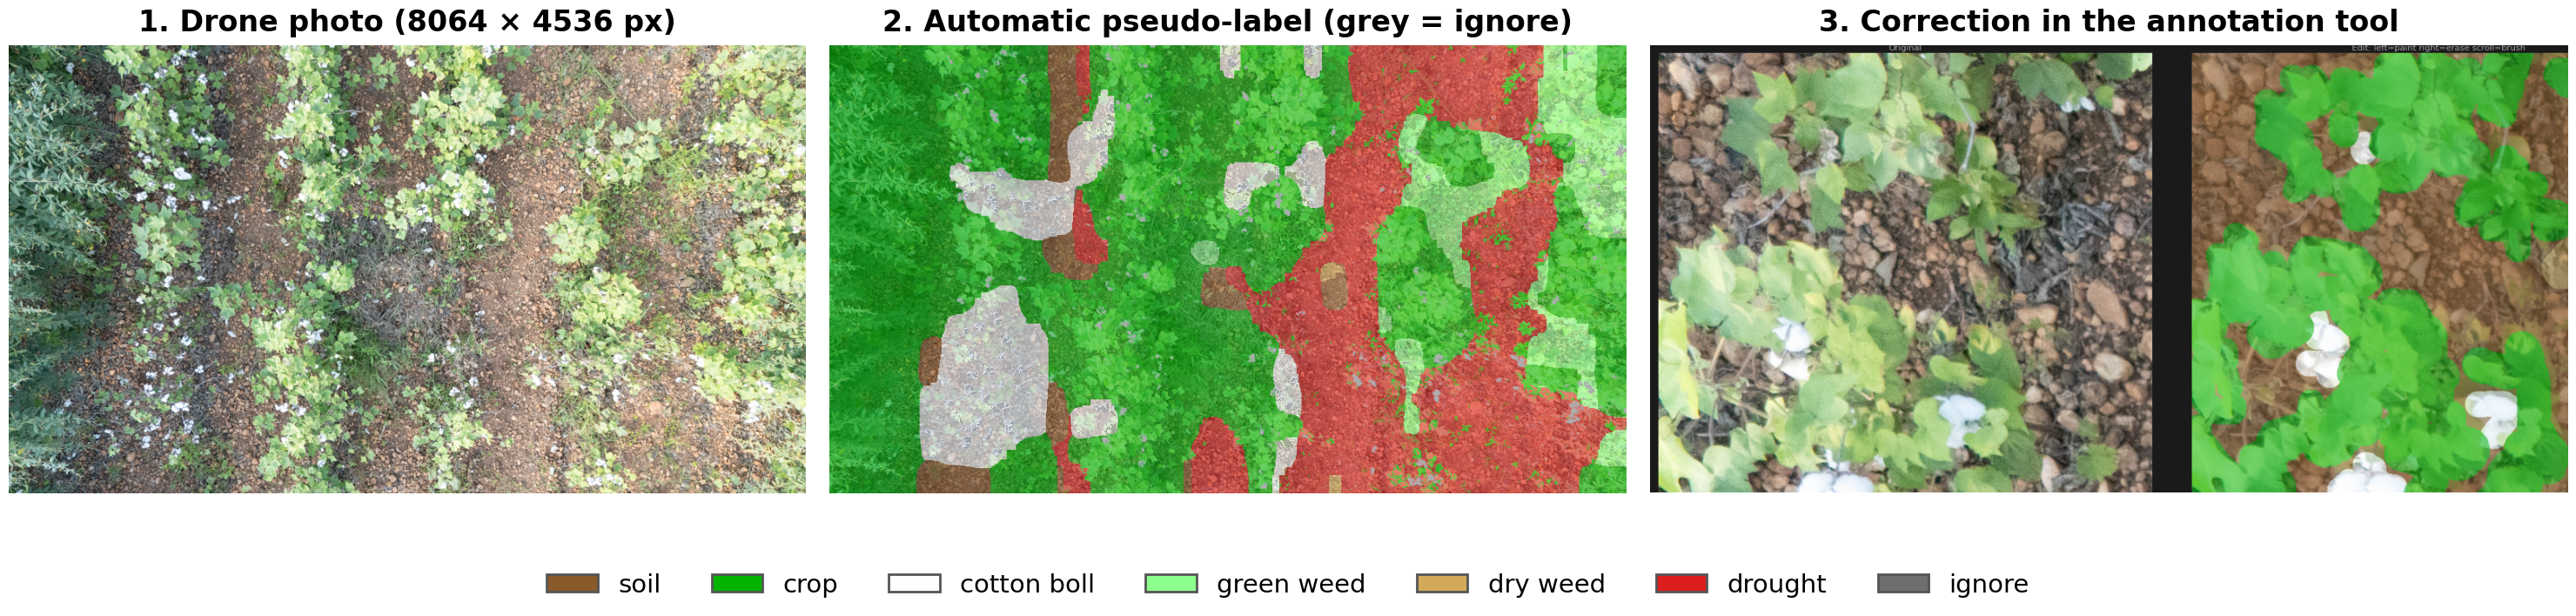
\includegraphics[width=0.80\textwidth]{figures/uav_step_labels.png}\\[0.5mm]
\begin{columns}[T]
\column{0.45\textwidth}
\begin{block}{Labels}
\scriptsize
\begin{itemize}
\item Pseudo-labels: 512\,px window, stride 256, dense CRF; confidence $< 0.55$ $\rightarrow$ ignore
\item Custom tool (Tkinter, Matplotlib, OpenCV): brush 2--150\,px, 50-step undo
\item \textbf{279 clean tiles} (224 train, 55 validation)
\item Per epoch: 500 clean + 500 pseudo + 1,000 synthetic (weights 8 / 0.5 / 1)
\end{itemize}
\end{block}
\column{0.53\textwidth}
\begin{block}{Nine channels (RGB in [0,1])}
\scriptsize
RGB (ImageNet-normalised) \;+\; $\tfrac{2G-R-B}{2}$ \;+\; $\tfrac{(2G-R-B)-(1.4R-G)}{3}$ \;+\; $-\tfrac{0.441R-0.811G+0.385B}{0.811}$\\[2pt]
+\; $\mathrm{GLI}=\tfrac{2G-R-B}{2G+R+B}$ \;+\; $\mathrm{NGRDI}=\tfrac{G-R}{G+R}$ \;+\; $V' = 2V-1$\\[2pt]
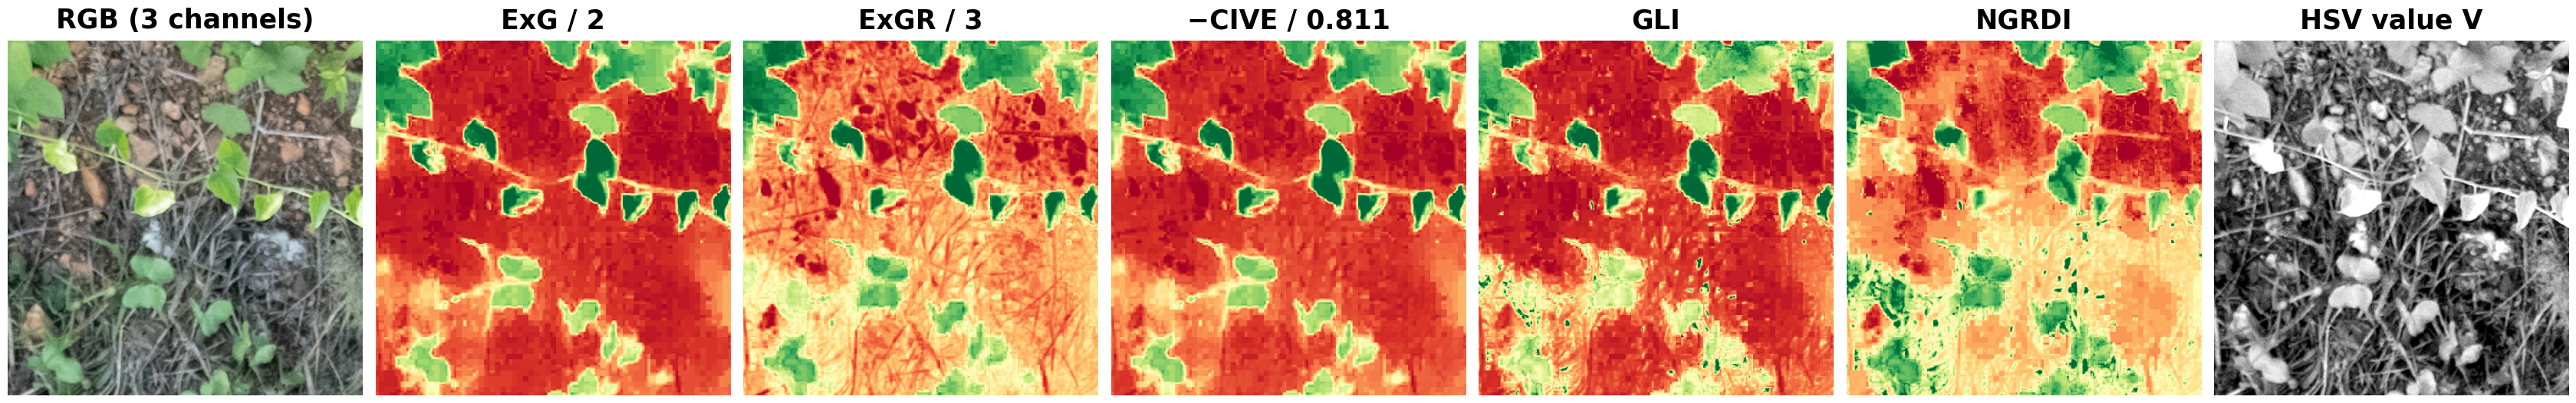
\includegraphics[width=\linewidth]{figures/uav_step_channels.png}
\end{block}
\end{columns}
\end{frame}

% ============================================================ 22 MODEL + TRAINING
\begin{frame}{7.5 Model and Training -- Nine-Channel SegFormer-B2}
\begin{columns}[T]
\column{0.60\textwidth}
\centering
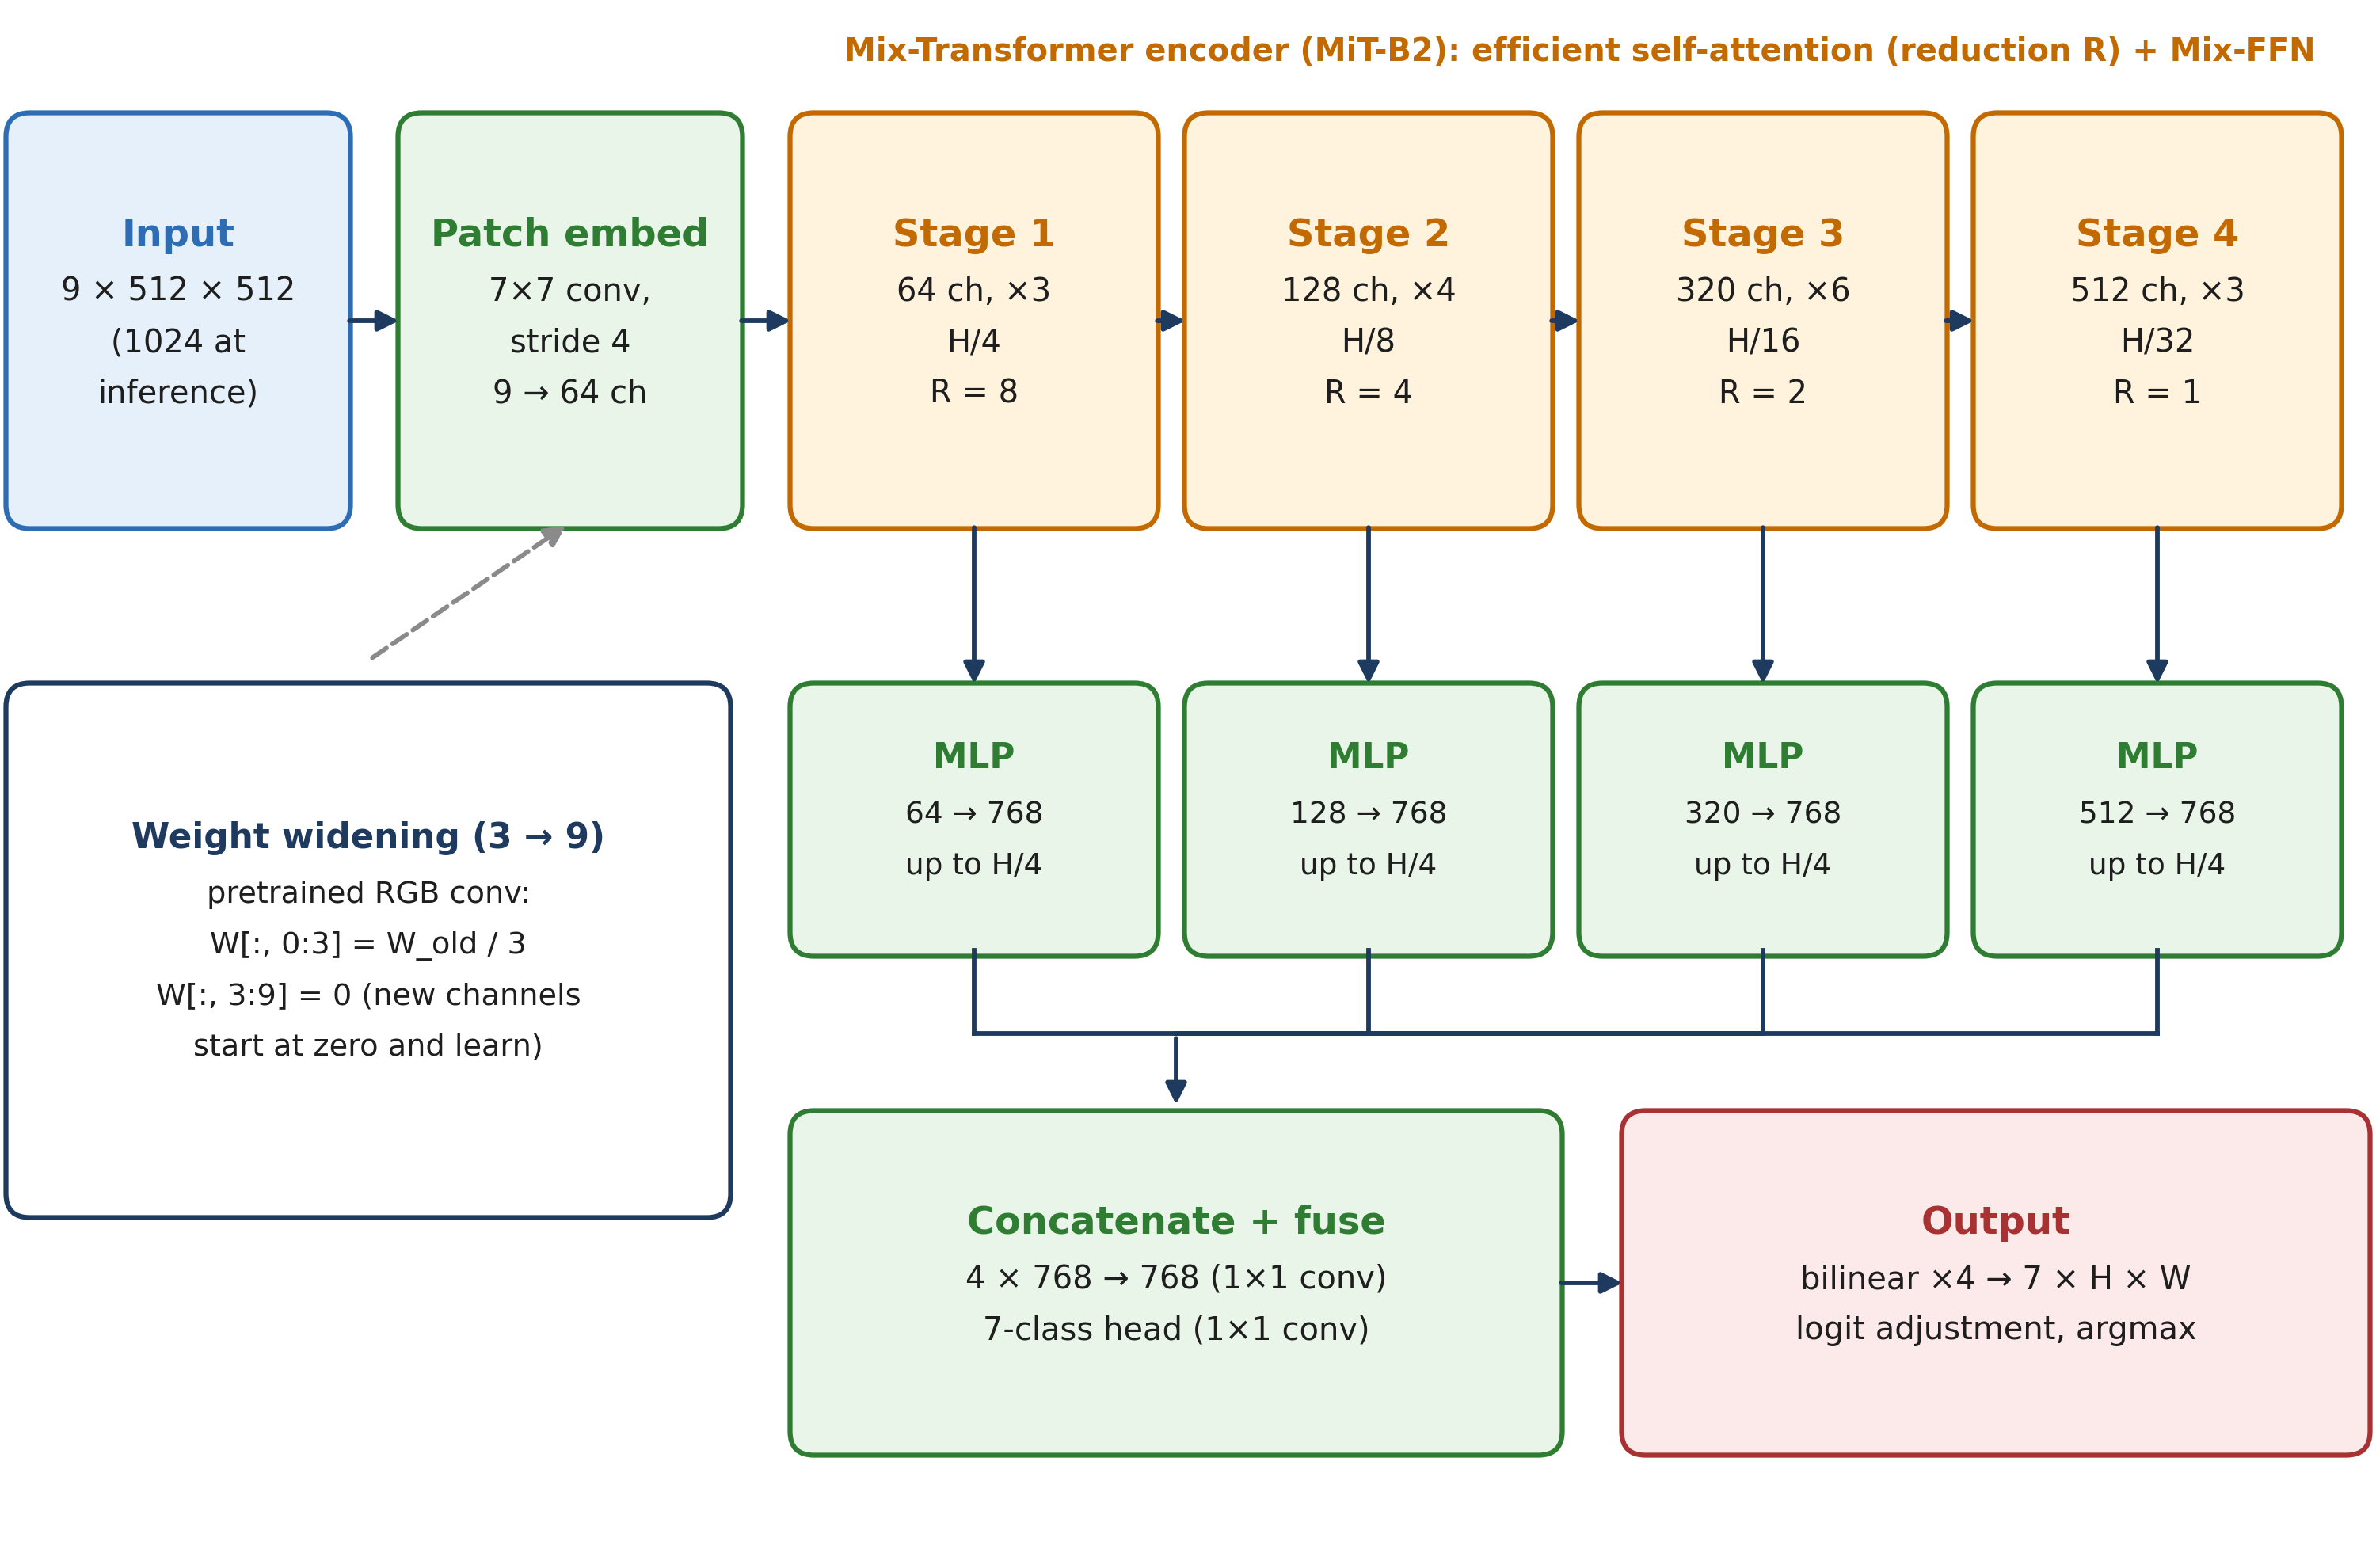
\includegraphics[width=0.86\linewidth]{figures/v2_uav_model.png}\\[1mm]
\begin{exampleblock}{Logit adjustment (chosen on validation tiles)}
\scriptsize Drought logit $-1.2$, dry-weed logit $-0.4$ $\Rightarrow$ drought precision \textbf{54.4\% $\rightarrow$ 76.4\%}, recall 95.5\% $\rightarrow$ 82.1\%, drought IoU \textbf{53.0\% $\rightarrow$ 65.5\%}.
\end{exampleblock}
\column{0.38\textwidth}
\begin{block}{Training}
\scriptsize
$\mathcal{L} = 1.0\,\mathcal{L}_{\text{focal}}(\gamma{=}2) + 2.5\,\mathcal{L}_{\text{Dice}} + 1.0\,\mathcal{L}_{\text{Lov\'asz}}$\\[2pt]
$\mathcal{L}_{\text{focal}} = -\alpha_y (1-p_y)^{\gamma}\log p_y$\\[2pt]
Class weights $\alpha_c = N/(C N_c)$, clipped to [0.1, 50]; drought 10, cotton boll 8.\\[2pt]
AdamW, lr $2\times10^{-6}$, cosine decay, batch 16, 10 epochs; best validation mIoU at epoch 5.
\end{block}
\begin{block}{Architecture}
\scriptsize Mix-Transformer encoder, 4 stages (64/128/320/512 channels, depths 3/4/6/3) at 1/4--1/32 resolution; MLP decoder (768) fuses all stages into 7-class logits, upsampled $\times4$. ImageNet-pretrained first convolution widened from 3 to 9 channels: $W_{\text{new}}[:,0{:}3] = W_{\text{old}}/3$, $W_{\text{new}}[:,3{:}9] = 0$.
\end{block}

\end{columns}
\end{frame}

% ============================================================ 23 STITCHING
\begin{frame}{7.6 Prediction Stitching, Area and Stress Decision}
\centering
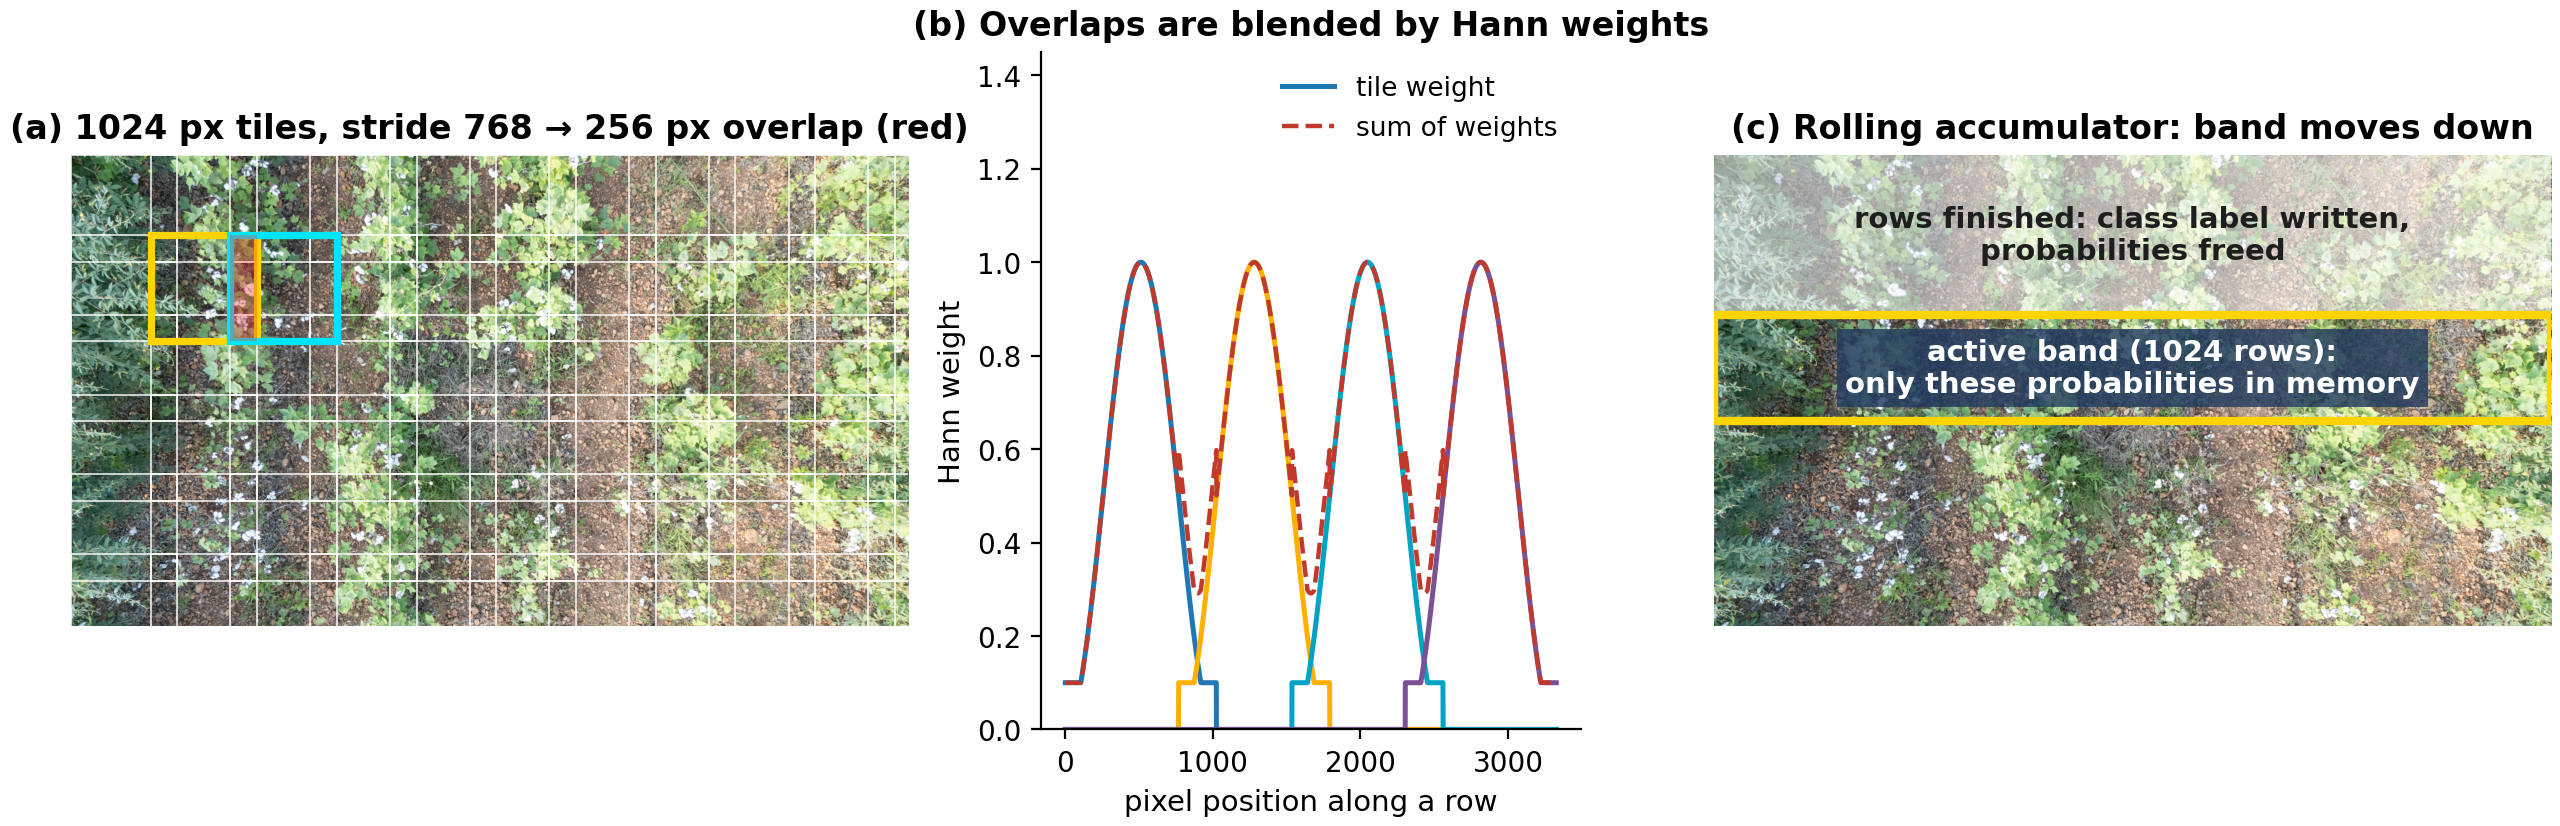
\includegraphics[width=0.85\textwidth]{figures/uav_step_stitching.png}\\[0.5mm]
\begin{columns}[T]
\column{0.5\textwidth}
\begin{block}{Seam-free, memory-safe stitching}
\scriptsize
$1024$\,px tiles, stride 768: \; $A_c(x) = \sum_i w_i(x)\,p_{i,c}(x)$, class $=\arg\max_c A_c(x)$\\
Rolling band: \textbf{1.5\,GB instead of 80\,GB} for a 2.86-billion-pixel orthomosaic.\\
Post-processing: no-data border, glare/shadow fix, small regions, harvest zones.
\end{block}
\column{0.48\textwidth}
\begin{block}{Area and visual stress flag}
\scriptsize
Area $= N_c \times (\mathrm{GSD}/1000)^2$ m$^2$.\\
$D$ = drought share of crop area, $N$ = same outside harvest zones, $C$ = share in the largest drought region.\\
\textbf{Flag} if $D > 0.15$ or ($N > 0.10$ and $C > 0.25$).
\end{block}
\end{columns}
\end{frame}

% ============================================================ 24 VALIDATION
\begin{frame}{7.7 UAV Validation Results (55 validation tiles)}
\begin{columns}[T]
\column{0.52\textwidth}
\scriptsize
\renewcommand{\arraystretch}{1.2}
\begin{tabular}{@{}lc@{}}
\toprule
\textbf{Model version} & \textbf{mIoU (\%)} \\ \midrule
V8, SegFormer-B2 & 61.18 \\
V9 / V9.1, SegFormer-B3 & 44.25 / 45.89 \\
V10, DeepLabV3+ & 44.79 \\
\textbf{V11, SegFormer-B2 (final)} & \textbf{61.46} \\
V12, SegFormer-B2 & 61.39 \\
\bottomrule
\end{tabular}\\[2pt]
\begin{exampleblock}{Final V11 (after logit adjustment)}
\footnotesize
\centering
\begin{tabular}{@{}c@{\hspace{6mm}}c@{\hspace{6mm}}c@{}}
{\color{navy}\bfseries\large 65.1\%} & {\color{navy}\bfseries\large 82.7\%} & {\color{navy}\bfseries\large 79.2\%} \\
{\scriptsize mIoU} & {\scriptsize pixel accuracy} & {\scriptsize drought F1}
\end{tabular}\\[2pt]\raggedright
\scriptsize Per-class IoU: soil 74, crop 73, cotton 53, green weed 71, dry weed 54, drought 65\%.
\end{exampleblock}
\begin{alertblock}{Honest note}
\scriptsize Validation, not an independent test: 22 of 55 tiles share source photos (source-disjoint tiles: 69.3\%); adjustment tuned on these tiles.
\end{alertblock}
\column{0.46\textwidth}
\centering
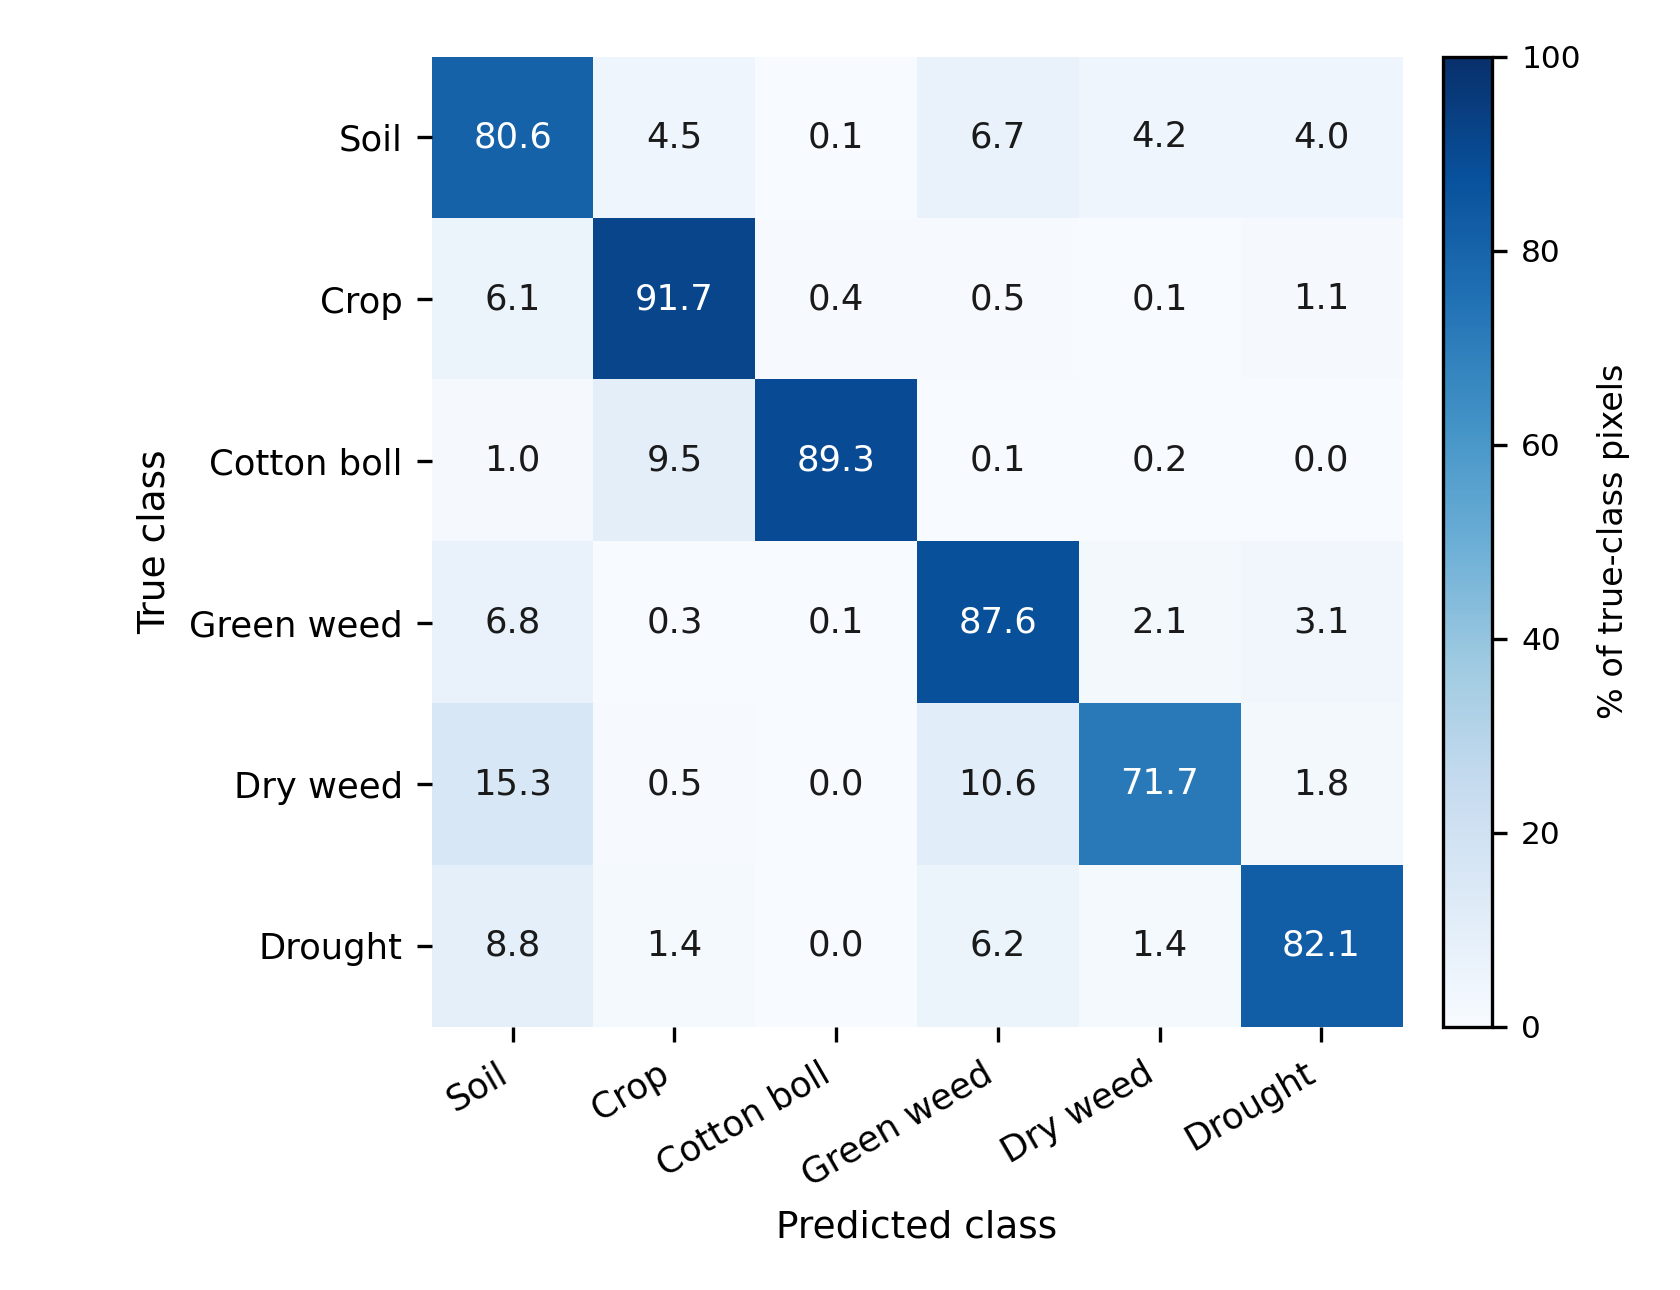
\includegraphics[height=0.66\textheight]{figures/uav_confusion.png}\\
{\scriptsize Row-normalised confusion matrix (\%)}
\end{columns}
\end{frame}

% ============================================================ 25 FIELD RESULTS
\begin{frame}{7.8 UAV Results on the 14 Fields}
\begin{columns}[T]
\column{0.52\textwidth}
\scriptsize
\renewcommand{\arraystretch}{1.15}
\begin{tabular}{@{}lrrrc@{}}
\toprule
\textbf{Field} & \textbf{GSD mm} & \textbf{Area m$^2$} & \textbf{Drought \%} & \textbf{Flag} \\ \midrule
Lepakshi & 2.08 & 2,976 & \textbf{71.53} & \textbf{yes} \\
Sira & 2.14 & 4,341 & \textbf{54.26} & \textbf{yes} \\
Somandepalle & 2.35 & 3,936 & \textbf{25.45} & \textbf{yes} \\
KNL Puddur & 1.73 & 3,866 & 0.15 & no \\
KNL Maize Tower & 1.68 & 2,241 & 0.07 & no \\
Pulliah & 2.69 & 2,897 & 0.04 & no \\
Balaji Villas & 1.84 & 8,044 & 0.06 & no \\
Shilpa & 1.94 & 6,395 & 0.00 & no \\
KNL DDP & 5.55 & 19,812 & 0.00 & no \\
Peddakadubur F1/F3/F4/F6/F7 & 3.6--18.5 & 42--660 & 0--0.89 & no \\
\bottomrule
\end{tabular}\\[2pt]
\begin{exampleblock}{Key finding}
\scriptsize The 3 flagged fields are exactly the southern fields the survey team judged drought-hit; no Kurnool field is flagged. Largest orthomosaic (2.86 billion px): 45 min on one L4 GPU.
\end{exampleblock}
\column{0.48\textwidth}
\centering
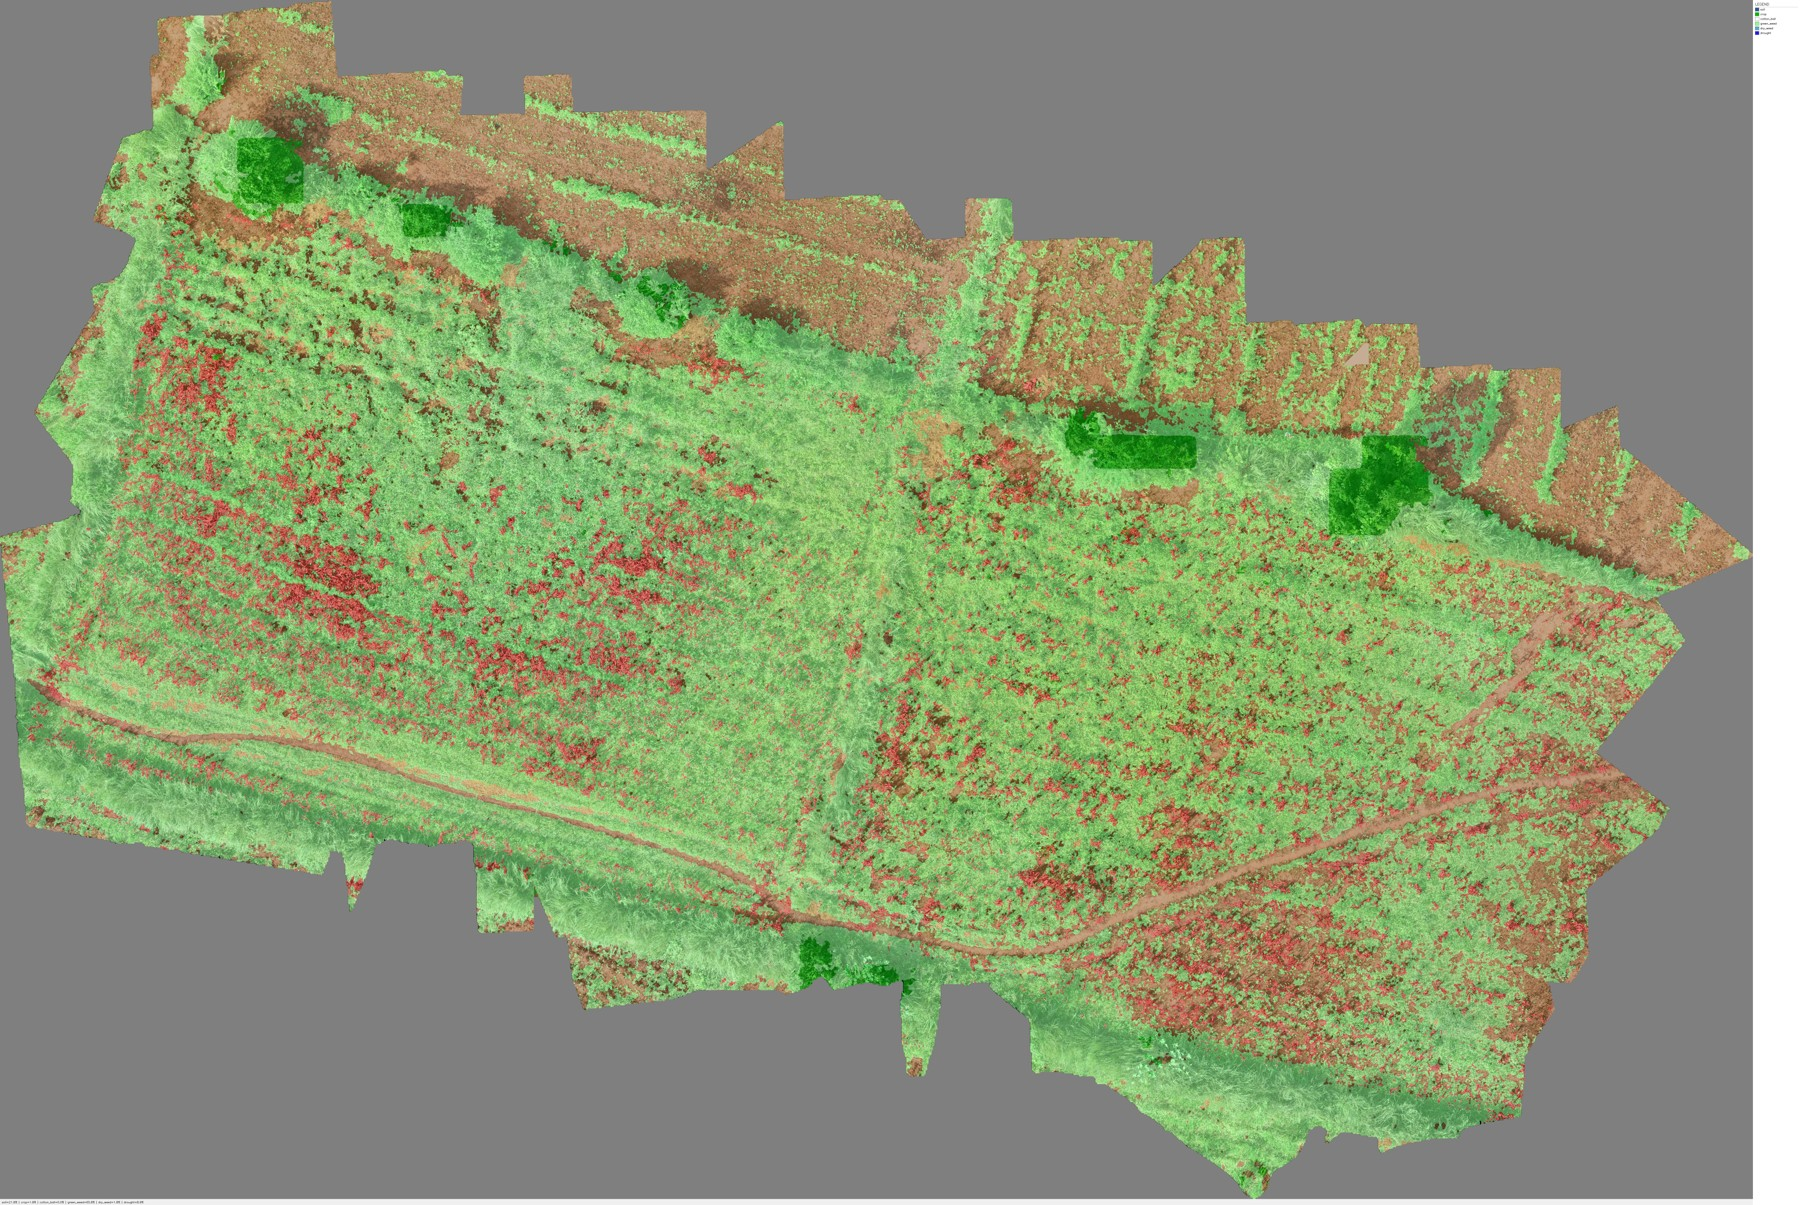
\includegraphics[height=3.1cm]{figures/uav_lepakshi_overlay.jpg}\\[1mm]
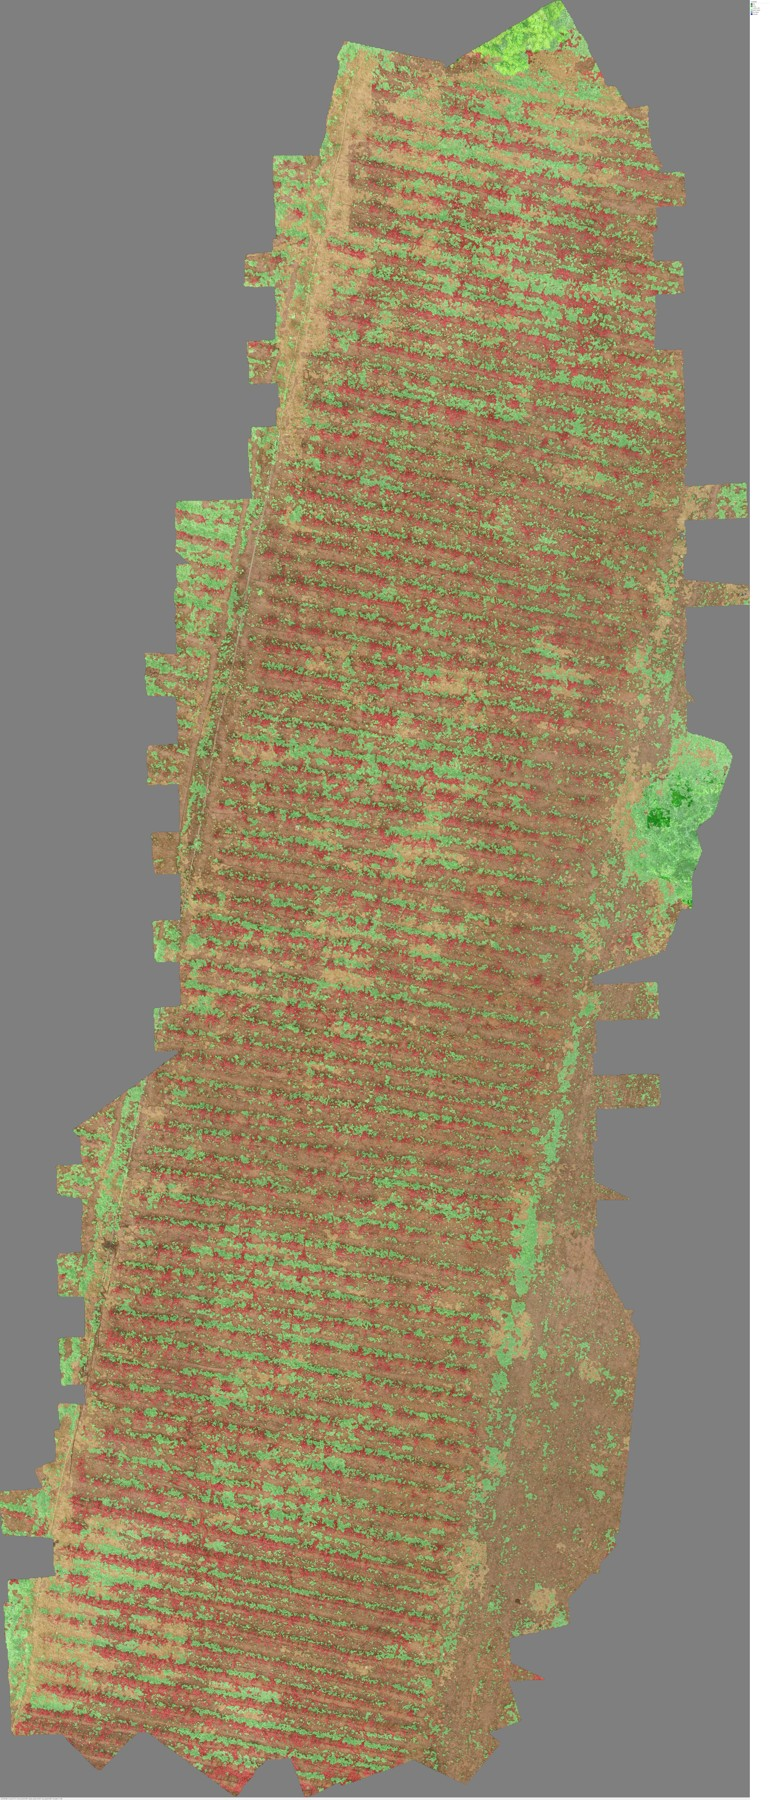
\includegraphics[height=2.9cm]{figures/uav_sira_overlay.jpg}\hspace{2mm}
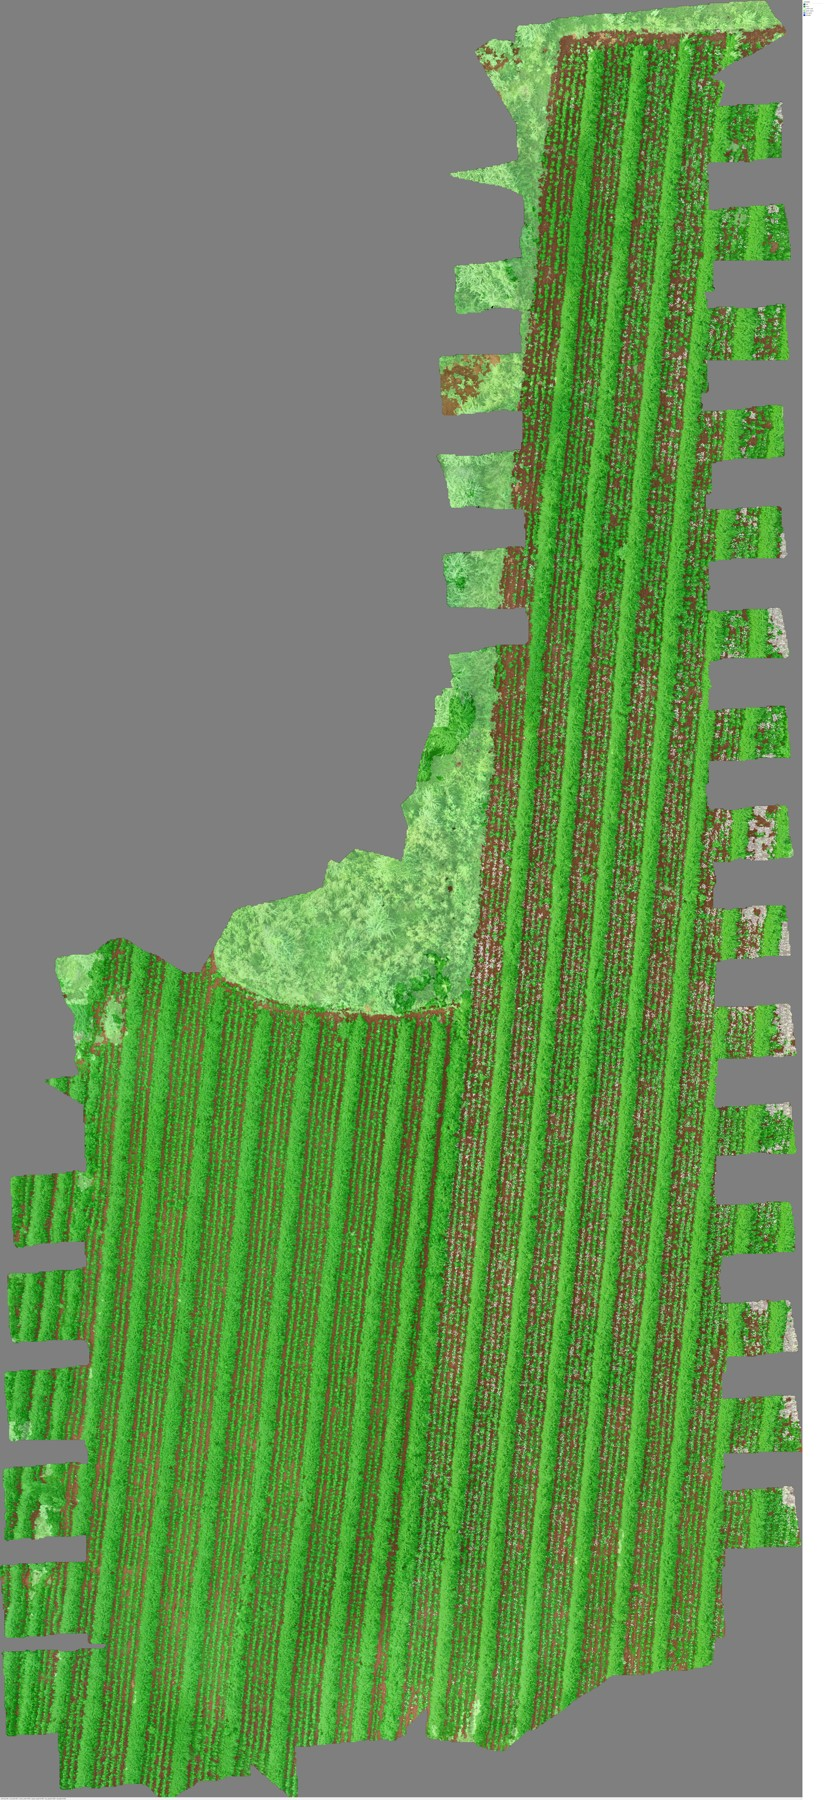
\includegraphics[height=2.9cm]{figures/uav_knlddp_overlay.jpg}\\
{\scriptsize Lepakshi (top), Sira (flagged) and KNL DDP (not flagged); red = drought}
\end{columns}
\end{frame}

% ============================================================ 26 CONCLUSION
\begin{frame}{8. Conclusion, Limitations and Future Work}
\begin{columns}[T]
\column{0.32\textwidth}
\begin{exampleblock}{Kharif}
\centering\key{9 / 9}{severe droughts confirmed, 5 before the order}\\[3pt]
\raggedright\scriptsize Hybrid weather forecast 0.819 / 0.651 at 7 / 15 days; crops respond about 10 days later.
\end{exampleblock}
\column{0.32\textwidth}
\begin{exampleblock}{Rabi}
\centering\key{AUC 0.80}{crop-loss warning by 15 December}\\[3pt]
\raggedright\scriptsize Confirmed by MODIS (0.83); soil-dry field warnings twice as reliable.
\end{exampleblock}
\column{0.32\textwidth}
\begin{exampleblock}{UAV}
\centering\key{65.1\% mIoU}{7-class maps of billion-pixel fields}\\[3pt]
\raggedright\scriptsize Flags the 3 fields the survey team judged drought-hit; 1.5\,GB instead of 80\,GB.
\end{exampleblock}
\end{columns}
\vspace{2mm}
\begin{columns}[T]
\column{0.49\textwidth}
\begin{alertblock}{Limitations}
\scriptsize
\begin{itemize}
\item No field-level drought ground truth; orders and yields are indirect
\item No skill 30 days ahead (kharif); few dry rabi test seasons
\item UAV: validation tiles only; RGB shows visual stress, not its cause
\end{itemize}
\end{alertblock}
\column{0.49\textwidth}
\begin{block}{Future work}
\scriptsize
\begin{itemize}
\item Run the full kharif / rabi $\rightarrow$ UAV loop in rabi 2026-27
\item Finish the 127-tile independent UAV test with field confirmation
\item Trend-robust greenness reference; multispectral / thermal drone imagery
\end{itemize}
\end{block}
\end{columns}
\end{frame}

% ============================================================ 27 REFERENCES
\begin{frame}{References}
\tiny
\begin{columns}[T]
\column{0.49\textwidth}
\begin{enumerate}\setlength{\itemsep}{1.5pt}
\item Govt.\ of India, \emph{Manual for Drought Management}, 2016 (updated 2020).
\item K.~Bhardwaj, V.~Mishra, ``Drought detection and declaration in India,'' \emph{Water Security}, 14, 2021.
\item S.~M.~Vicente-Serrano \emph{et al.}, ``A multiscalar drought index sensitive to global warming: the SPEI,'' \emph{J.\ Climate}, 23(7), 2010.
\item A.~Dikshit, B.~Pradhan, A.~Huete, ``An improved SPEI drought forecasting approach using the LSTM,'' \emph{J.\ Environ.\ Manage.}, 283, 2021.
\item A.~Marusov \emph{et al.}, ``Long-term drought prediction using deep neural networks based on geospatial weather data,'' \emph{Environ.\ Model.\ Softw.}, 179, 2024.
\item A.~Belayneh \emph{et al.}, ``Long-term SPI drought forecasting \ldots\ wavelet neural network and wavelet SVR,'' \emph{J.\ Hydrology}, 508, 2014.
\item H.~Boogaard \emph{et al.}, ``AgERA5,'' Copernicus Climate Data Store.
\item F.~N.~Kogan, ``Application of vegetation index and brightness temperature for drought detection,'' \emph{Adv.\ Space Res.}, 15(11), 1995.
\item A.~J.~Peters \emph{et al.}, ``Drought monitoring with NDVI-based Standardized Vegetation Index,'' \emph{PE\&RS}, 68(1), 2002.
\item S.~Park \emph{et al.}, ``Drought assessment and monitoring through blending of multi-sensor indices using machine learning,'' \emph{Agric.\ Forest Meteorol.}, 216, 2016.
\item S.~S.~Sharma \emph{et al.}, ``Leveraging Sentinel-2 data and machine learning for drought detection in India,'' \emph{Remote Sens.}, 17(18), 2025.
\item N.~Gorelick \emph{et al.}, ``Google Earth Engine,'' \emph{Remote Sens.\ Environ.}, 202, 2017.
\end{enumerate}
\column{0.49\textwidth}
\begin{enumerate}\setcounter{enumi}{12}\setlength{\itemsep}{1.5pt}
\item S.~K.~Padhee \emph{et al.}, ``Integrating EDI and remote sensing derived parameters for agricultural drought assessment in Bundelkhand,'' \emph{ISPRS Arch.}, XL-8, 2014.
\item B.~R.~Nikam \emph{et al.}, ``Assessment of early season agricultural drought using remote sensing,'' \emph{ISPRS Arch.}, XLIII-B3, 2020.
\item A.~Descals \emph{et al.}, ``Evaluating Sentinel-2 for monitoring drought-induced crop failure in winter cereals,'' \emph{Remote Sens.}, 17(2), 2025.
\item J.~Pang \emph{et al.}, ``Pattern of water use and seed yield under terminal drought in chickpea,'' \emph{Front.\ Plant Sci.}, 8, 2017.
\item E.~Xie \emph{et al.}, ``SegFormer: simple and efficient design for semantic segmentation with Transformers,'' \emph{NeurIPS}, 2021.
\item T.~B.~Shahi \emph{et al.}, ``Classification of water stress in cotton using CNNs from UAV images,'' \emph{Remote Sens.}, 15(1), 2023.
\item F.~Dang \emph{et al.}, ``Deep learning-based weed detection using UAV images: a comparative study,'' \emph{Drones}, 7(1), 2023.
\item M.~Berman \emph{et al.}, ``The Lov\'asz-Softmax loss,'' \emph{CVPR}, 2018.
\item T.-Y.~Lin \emph{et al.}, ``Focal loss for dense object detection,'' \emph{ICCV}, 2017.
\item R.~Achanta, S.~S\"usstrunk, ``Superpixels and polygons using simple non-iterative clustering,'' \emph{CVPR}, 2017.
\end{enumerate}
\end{columns}
\end{frame}

% ============================================================ 28 THANK YOU
\begin{frame}[plain]
\centering
\vspace{8mm}

\includegraphics[height=2.0cm]{figures/logo.jpeg}\\[5mm]
{\fontsize{34}{38}\selectfont\color{navy} Thank You}\\[5mm]
{\large A Multimodal Framework for Agricultural Drought Monitoring and Prediction}\\[3mm]
{\normalsize Weather Time Series \;$|$\; Satellite Imagery \;$|$\; UAV Semantic Segmentation}\\[5mm]
{\footnotesize Department of Computer Science and Engineering\\
Indian Institute of Information Technology Design and Manufacturing Kurnool}
\end{frame}

\end{document}
